%\chapter{Recuperação automatizada da informação corporativa e facetada} - manter comentado

	\begin{flushright}
		\textit{``Há apenas um bem, o saber; \\e apenas um mal, a ignorância''.\\
		Sócrates}
	\end{flushright}


%\textbf{Introdução do capítulo.}
Este capítulo apresenta dois experimentos de recuperação de informação corporativa que se utilizam das coleções particular e pública de documentos corporativos analisadas. 

%\textbf{Introdução ao primeiro experimento.}
No primeiro experimento foi observado como os usuários de informação da coleção particular constroem as expressões de busca e quais características são compartilhadas entre as expressões de busca e os documentos da coleção particular. Essa é a mesma estratégia adotada para análise e representação do domínio corporativo, descrita no capítulo \ref{analiseDominio}, mas desta vez realizada com um conjunto de usuários de informação em seu contexto de trabalho.

%\textbf{Razão do primeiro experimento e diferença do experimento padrão da literatura.}
Esta pesquisa não dispensou uma avaliação complementar àquela predominante na literatura, com a coleção particular e usuários reais, para garantir que os resultados realmente retratem as influências das características específicas da informação corporativa nos métodos de recuperação de informação em situações mais próximas da realidade corporativa. Sua principal diferença é a importância dada à análise de domínio como componente formal da construção da coleção particular, o estabelecimento dos contextos de uso mais úteis para os usuários de informação e o reconhecimento das características mobilizadas e adotadas por usuários e produtores de informação \cite{lykke2011domain}.

%\textbf{Limitação do primeiro experimento.}
Porém, embora pretenda validar as conclusões desta tese, o primeiro experimento esbarra na dificuldade de reunir usuários de informação com as mesmas características daqueles que observamos em outras empresas, e na dificuldade de ter acesso direto aos usuários de informação. Portanto, a repetibilidade dos experimentos é comprometida e o problema deve ser amenizado com a execução de experimentos adicionais.

%\textbf{Introdução ao segundo experimento.}
No segundo experimento foi implementado um protótipo de sistema de recuperação de informação corporativa (SRIC) com componentes adaptados para indexar e recuperar informação facetada. Esse segundo experimento objetivou explicitar como a organização facetada da informação influencia os diferentes componentes do SRIC. O segundo experimento fez uso dos documentos da coleção de referência da trilha \textit{Enterprise} da \textit{Text Retrieval Conference}. Também fez uso do modelo de avaliação da eficiência de indexação e recuperação \cite{balog08}, reconhecido na literatura como avaliação de \textit{Cranfield}.

%\textbf{Motivo para o segundo experimento.}
A presença de uma coleção de referência favorece a comparação de trabalhos e a definição de bases de comparação. O contrário, quando experimentos são realizados em coleções particulares, a publicação de resultados se baseia muitas vezes em informação protegida, não disponível publicamente e muitas vezes sensível. Há muitas metodologias de avaliação de sistemas de recuperação de informação \cite{irEvaluation02,evaluationWithIncompleteInformation04,bucher05,sakai08ret,DBLP:conf/clef/2008}, algumas delas bem aceitas na indústria e na academia. Porém, há limitações para avaliação de sistemas corporativos pelas mesmas metodologias, dadas suas especificidades \cite{craswell05}.

%\textbf{Limitação do segundo experimento.}
Na avaliação de \textit{Cranfield} para informação corporativa, os critérios de relevância, coleções de referência e métricas de desempenho não parecem adequados para avaliar como diferentes atores sociais recuperam informação corporativa nos mais diversos contextos de uso. Entretanto, este trabalho adotou os procedimentos e resultados de \citeonline{bailey07} e \citeonline{balog08} como base de comparação, mas reconhece a impossibilidade de concluir que aperfeiçoamentos arbitrários em um sistema de recuperação de informação, mesmo bem-sucedidos sobre a coleção pública, sejam eficientes para toda e qualquer empresa. Mesmo com essa limitação, esta tese procura interpretar a razão do sucesso e do insucesso de algumas estratégias de recuperação, usadas aqui e na literatura que baseia-se na trilha \textit{Enterprise}.

%\textbf{Link para as próximas seções.}
Os resultados sobre a coleção particular são apresentados na seção \ref{prototipo-colecaoParticular} e os resultados sobre a coleção pública são apresentados na seção \ref{prototipo-colecaoPublica}. As discussões dos resultados ocorrem isoladamente dentro das seções citadas em função das especificidades de cada experimento.









\section{Experimento sobre a coleção particular}
\label{prototipo-colecaoParticular}

%\subsection{Procedimentos metodológicos}

%\textbf{Caracterização do primeiro experimento.}
No primeiro experimento, os procedimentos metodológicos empreendidos cumpriram a função de caracterizar os documentos de uma coleção corporativa e as consultas de usuários ao buscar por um conjunto de documentos. A coleção de documentos adotada é um conjunto de documentos escritos em língua portuguesa, pertencente a um campus do Centro Federal de Educação Tecnológico de Minas Gerais (CEFETMG), em Timóteo, Minas Gerais. São 1305 documentos que incluem principalmente e-mails, páginas Web, relatórios técnicos, notícias internas e externas, e pautas e atas de reunião. Os documentos foram criados entre os anos de 2007 e 2013 e têm sido acessados por seus usuários durante o período de 2012 a 2013. Esses são os mesmos documentos usados na análise preliminar de domínio apresentada no capítulo anterior.

%\textbf{Caracterização da participação.}
De uma população de sete coordenadores, cinco se prontificaram a participar da pesquisa. Eles são familiarizados com o uso dos documentos da coleção e foram solicitados a propor expressões de busca, denominadas também como simplesmente consultas neste capítulo, que levassem para os mesmos dez documentos da coleção de documentos, pré-selecionados aleatoriamente.

%\textbf{Caracterização dos participantes.}
Os cinco participantes foram coordenadores durante o período de 2007 a 2014 ou são coordenadores atualmente. Todos são professores do sexo masculino, sendo que dois deles pertencem à área de Engenharia Elétrica e três à área de Ciência da Computação. Dois concluíram o doutorado e três concluíram o mestrado antes de exercerem o cargo.

%\textbf{Ambiente da participação.}
A proposta de participação na pesquisa foi enviada através do e-mail profissional. A mensagem do e-mail trazia a proposta da pesquisa, seu formato e aspectos éticos, as instruções, exemplos de consulta e o endereço do formulário on-line através do qual as consultas deveriam ser registradas. A mensagem original encontra-se disponível no anexo \ref{anexoMensagem}. A mensagem incluiu onze documentos, um usado para algumas consultas de exemplo que simplesmente ilustravam o que constituía uma expressão de consulta, e dez que compõem a amostra. Os participantes registraram as consultas sem usar \textit{softwares} ou repositórios da empresa, tendo acesso irrestrito à Internet. Responderam a pesquisa quando estavam em casa, sem prazo limite de participação, através de um formulário eletrônico como ilustrado no anexo \ref{anexoQuestionario}.

%\textbf{Definição da amostra de documentos a recuperar.}
A escolha de documentos foi aleatória por não haver qualquer indício de vício na coleção, supostamente composta apenas por documentos conhecidos e úteis para a unidade organizacional. O número de documentos, por outro lado, foi decidido considerando a utilidade para a pesquisa e a viabilidade para os participantes. Era esperado que um número reduzido de documentos permitisse aos participantes realizar as consultas de uma única vez, sem que a participação fosse interrompida por obrigações profissionais ou domésticas.

%\textbf{Condições para consulta.}
A consulta proposta deveria ser escrita em linguagem natural, uma vez que não há vocabulário controlado para aqueles documentos. No entanto, como cada documento de interesse era consultado antes da elaboração de sua consulta, era esperado que o vocabulário presente no documento fosse adotado por todos os participantes.

%\textbf{Requisitos do experimento.}
Para reduzir algumas das limitações do método e permitir pesquisas que possam ser comparadas com a atual, os seguintes requisitos foram definidos: a amostra de documentos é aleatória; uma cópia dos documentos foi entregue aos participantes, dispensando-os de acessar qualquer repositório da empresa; os participantes foram instruídos a não usarem qualquer recurso além dos documentos providos; não foi fornecida orientação sobre como se fazer uma busca eficiente ou quais e quantos termos deveriam ser usados na consulta; e os participantes foram orientados a consumirem o tempo de dez minutos para elaborar todas as consultas.

%\textbf{Descarte de um dos formulários.}
Um dos participantes é autor desta tese e foi o responsável pela categorização dos documentos da coleção. Portanto, como o objetivo deste trabalho é comparar características dos documentos e das consultas dos usuários, seu formulário foi descartado e os resultados da pesquisa não usam as consultas propostas pelo autor. Sua participação serviu apenas para testar o formulário e estimar o tempo de resposta.

%\textbf{Análise de assunto e análise facetada sobre as expressões de busca.}
Foi feita a análise de assunto e posteriormente aplicada a análise facetada para a determinação das facetas  nas consultas de quatro participantes, totalizando 40 consultas. Como visto no capítulo anterior, os documentos foram indexados e categorizados por um único pesquisador. A indexação produziu uma lista de termos em linguagem natural que pertencem à coleção, tendo sido categorizados ao final da indexação. São as categorias e dois níveis de subcategorias os objetos de estudo neste trabalho, sendo que nem sempre os três níveis foram mobilizados. Um exemplo de termo em que apenas um nível foi mobilizado é ‘denúncia’, categorizado como Comunicação. O termo ‘departamento’ mobiliza dois níveis, a categoria Instituição e a subcategoria Unidade. O termo ‘diretor’, por sua vez, mobiliza os três níveis, a categoria Pessoal, a subcategoria Profissional e o terceiro nível Papel.

%\textbf{Explicação sobre a comparação empreendida entre as expressões de busca e os documentos.}
As categorias e subcategorias resultantes foram usadas para comparar as características dos assuntos que compõem o conteúdo dos documentos e o conteúdo das consultas dos usuários corporativos, respondendo aos objetivos deste capítulo. Para avaliar o padrão da distribuição de assuntos entre coleção e consultas foi adotado o coeficiente de correlação de Spearman. Ele se mostrou adequado para a comparação, além de não requerer uma análise estatística excessivamente complexa. Portanto, o coeficiente de Spearman também é útil para que os resultados presentes e de trabalhos futuros sejam comparados sem que os dados de empresas sejam expostos.

\subsection{Resultados do experimento sobre a coleção particular}
\label{prototipo-resultados-particular}

%\textbf{Introdução aos resultados.}
O principal objetivo deste primeiro experimento foi identificar as categorias ou características comuns a documentos corporativos e consultas de usuários enquanto buscam por documentos pertinentes em seu contexto de trabalho. Para isso, dez expressões de busca foram produzidas por quatro participantes da empresa investigada, totalizando 40 consultas. O tempo médio de produção de cada consulta foi igual a 1 minuto. A categorização dos termos presentes nas consultas foi realizada pelo mesmo indexador dos documentos, o que consumiu um tempo adicional de 2 horas e 22 minutos.

\begin{figure}
	\caption{\label{fig:avaliacaoPart-distribuicaoAssuntos}Distribuição de assuntos entre as categorias}

	\centering
		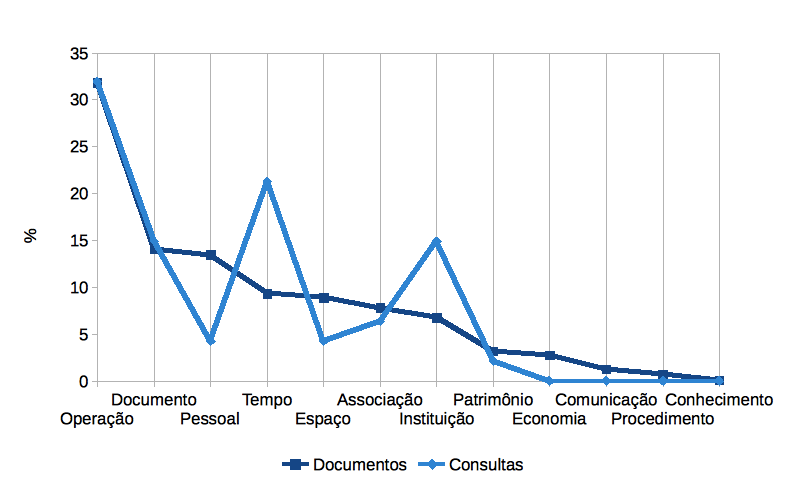
\includegraphics[width=1.0\textwidth]{fig/avaliacaoPart-distribuicaoAssuntos.png}

	\legend{Fonte: elaborada pelo autor}
\end{figure}

%\textbf{Assuntos encontrados na expressão de busca e compatibilidade da distribuição entre assuntos.}
O indexador identificou 1643 termos/assuntos diferentes em toda a coleção de documentos e 47 termos/assuntos diferentes nas consultas de usuários. Os assuntos identificados durante a indexação dos documentos e na formulação de consultas foram agrupados nas 12 categorias descobertas no capítulo \ref{analiseDominio}. A figura \ref{fig:avaliacaoPart-distribuicaoAssuntos} apresenta as categorias e a proporção de assuntos associados a cada uma delas. As categorias são Pessoal, Associação, Instituição, Documento, Comunicação, Economia, Conhecimento, Operação, Procedimento, Espaço, Patrimônio e Tempo. A proporção de assuntos em cada categoria é compatível entre a coleção de documentos e nas consultas formuladas por usuários da informação corporativa. As categorias que apresentaram maior compatibilidade entre os conjuntos avaliados são Operação, Documento, Associação e Patrimônio, com a frequência de assuntos quase idêntica entre documentos e consultas. As categorias Economia, Comunicação, Procedimento e Conhecimento, embora apresentem graficamente pontos próximos na figura \ref{fig:avaliacaoPart-distribuicaoAssuntos}, não apresentaram qualquer assunto nas consultas formuladas e portanto devem ser descartados da análise.

%\textbf{Demonstração da correlação via gráfico e via coeficiente.}
A figura \ref{fig:avaliacaoPart-correlacaoDistribuicaoAssuntos} ilustra a dispersão das frequências de assuntos em cada categoria entre os documentos e as consultas de seus usuários. A distribuição apresenta alta correlação positiva indicada por coeficiente de Spearman: $\rho(10) = 0,860912, n = 12, p = 0,0003231$, usando as 12 categorias de mais alto nível.

%\textbf{Inexistência de correlação nos níveis mais baixos.}
Por outro lado, nos níveis mais baixos da categorização, houve uma reduzida correlação positiva entre a distribuição de assuntos em facetas e subfacetas entre os documentos e as consultas. Isso sugere a inexistência de correlação estatística na medida em que o nível de classificação torna-se mais preciso.

\begin{figure}
	\caption{\label{fig:avaliacaoPart-correlacaoDistribuicaoAssuntos}Correlação da distribuição de assuntos entre categorias}

	\centering
		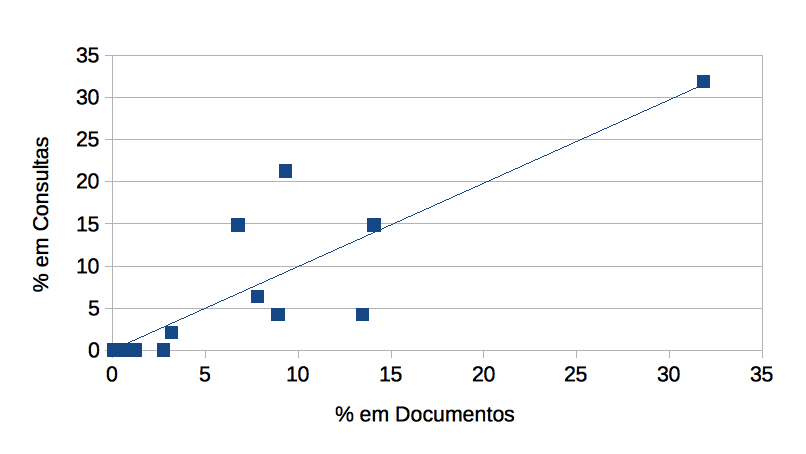
\includegraphics[width=1.0\textwidth]{fig/avaliacaoPart-correlacaoDistribuicaoAssuntos.png}

	\legend{Fonte: elaborada pelo autor}
\end{figure}

%\textbf{Apresentação da tabela e explicações.}
Analisando exclusivamente as expressões de busca, os usuários participantes fizeram uso de um total de 47 termos diferentes para elaborar as consultas que levariam aos dez documentos de interesse. A tabela \ref{termosUsuariosColecaoParticular} apresenta os termos adotados pelos usuários para os dez documentos da amostra. Para cada documento, os termos usados pelos usuários que pertencem a mesma categoria foram alinhados horizontalmente. Assim, para buscar pelo documento 1, os quatro usuários fizeram uso dos termos “congregação” e “ata” das categorias Operação e Documento. Apenas dois fizeram uso do termo “2009” e um fez uso do termo “dezembro de 2009”, ambos da categoria Tempo. Três deles fizeram uso do termo “timóteo” da categoria Espaço e “cefet” de Instituição. Dois deles fizeram uso do termo “reunião” da categoria Operação. Finalmente, apenas um deles fez uso do termo “campus” da categoria Instituição.




%\scriptsize
\begin{center}
%\begin{longtable}{p{4cm}|l|l|l|l}
\begin{longtable}{c|p{3cm}|p{3cm}|p{3cm}|p{3cm}}
\caption[Termos usados em expressões de busca de usuários da coleção particular]{Termos usados em dez expressões de busca de quatro usuários da coleção particular}
\label{termosUsuariosColecaoParticular}

\hline \textbf{Doc.} & \textbf{Usuário 1} & \textbf{Usuário 2} & \textbf{Usuário 3} & \textbf{Usuário 4}  \\ \hline 
\endfirsthead

\multicolumn{5}{c}%
{{\bfseries \tablename\ \thetable{} -- continuação da página anterior}} \\
\hline \textbf{Doc.} & \textbf{Usuário 1} & \textbf{Usuário 2} & \textbf{Usuário 3} & \textbf{Usuário 4} \\ \hline 
\endhead

\hline \multicolumn{5}{r}{{Continua na próxima página}} \\ \hline
\endfoot

%\hline % Retirada para incluir Fonte.
\endlastfoot

1 & congregação \newline\newline
ata \newline
2009 \newline\newline
timóteo \newline
cefet \newline
campus \newline
reunião
 & 
congregação \newline\newline
ata \newline
dezembro de 2009
 & 
congregação \newline\newline
ata \newline
 \newline\newline
timóteo \newline
cefet
 &
congregação unidade \newline
ata \newline
2009 \newline\newline
timóteo \newline
cefet \newline
 \newline
reunião
  \\ \hline

2 & regime disciplinar discente & regime disciplinar discente & 
regime disciplinar \newline\newline
cefet \newline
timóteo
 & 
regime disciplinar discente \newline
cefetmg
 \\ \hline

3 & 
palestra \newline
edificações \newline\newline
timóteo \newline
 \newline
2010
 & 
palestra\newline
edificações\newline\newline
\newline
\newline
\newline
incêndio
  & 
palestra\newline
\newline\newline
timóteo\newline
cefet\newline
\newline
combate incêndio
  & 
palestra\newline
curso técnico edificações\newline
timóteo\newline
cefet\newline
\newline
fundamentos para elaboração projeto prevenção
 \\ \hline

4 &
greve\newline
\newline
professor\newline
\newline
publicação externa\newline
2012
 &
greve\newline
timóteo\newline
professor
 &
greve\newline
timóteo\newline
\newline
cefet\newline
\newline\newline
\newline
diário do aço
 &
timóteo\newline
\newline\newline
cefet\newline
\newline
\newline\newline
\newline
dois meses de paralisação
 \\\hline

5 &
estrutura organizacional\newline
timóteo\newline
\newline
2014
 &
organograma\newline\newline
timóteo
 &
estrutura organizacional\newline
timóteo\newline
cefet
 &
estrutura organizacional\newline
timóteo\newline
cefet
 \\\hline

6 &
requerimento\newline
coordenação de programa de estágios
 &
requerimento\newline
\newline
\newline\newline\newline
\newline
estágio\newline
carta
 &
requerimento\newline
\newline\newline\newline
cefet\newline
timóteo\newline
estágio
 & 
requerimento\newline
coordenação programa estágio\newline\newline
cefet\newline
timóteo
 \\\hline

7 &
\newline
curso\newline\newline
pró-técnico\newline
2009\newline
\newline
\newline
\newline
publicação externa
  &
vestibular\newline
\newline\newline
pró-técnico\newline
2010
 & 
vestibular\newline
\newline
\newline\newline
\newline
prefeitura\newline
timóteo\newline
cefet
 & 
vestibular\newline
curso preparatório\newline
\newline
\newline
prefeitura\newline
timóteo\newline
cefet
 \\\hline

8 & 
fórum dos coordenadores\newline
ata\newline
\newline
\newline
\newline
recuperação\newline
sistema
 & 
fórum\newline\newline
ata\newline
março de 2013
 & 
fórum\newline\newline
ata\newline
\newline
cefet\newline
timóteo
 & 
fórum coordenadores\newline
ata\newline
2013\newline
cefet\newline
timóteo\newline
\newline
\newline
2\newline
reunião
 \\\hline

9 & 
palestra\newline
mark\newline
\newline
\newline
2013\newline
realidade aumentada
 & 
palestra\newline
mark
 & 
palestra\newline
mark\newline
cefet\newline
timóteo
 & 
palestra\newline
mark\newline
cefet\newline
timóteo\newline
\newline
\newline\newline
prof
 \\\hline

10 & 
congresso\newline
abm\newline
\newline
\newline
curso técnico em metalurgia
 & 
congresso\newline
abm\newline
\newline
expominas
 & 
congresso\newline
abm\newline
cefet\newline
timóteo
 & 
congresso\newline
abm\newline
cefet\newline
timóteo\newline
\newline\newline
64
 \\\hline

 \hline \multicolumn{5}{l}{Fonte: Elaborada pelo autor.}

\end{longtable}
\end{center}
%\normalsize






%\textbf{Apresentação do número de termos das 10 consultas.}
As consultas apresentaram grandes diferenças entre si. A consulta 1 foi formulada com o maior número de termos, 5 em média, e com o maior desvio-padrão 1,825. A consulta 2, por sua vez, foi formulada com o menor número de termos, 1,75 em média. Como um todo, as consultas foram formuladas com um número médio de termos igual 3,625, com desvio-padrão de 1,314. As discussões de resultados deste experimento são apresentadas na seção \ref{prototipo-discussoes-particular}.







\subsection{Discussões de resultados sobre a coleção particular}
\label{prototipo-discussoes-particular}

%\textbf{Introdução da seção.}
A seção \ref{prototipo-resultados-particular} apresentou os resultados da categorização de assuntos dos documentos corporativos e das consultas formuladas pelos usuários da coleção particular pesquisada. Os resultados atendem ao objetivo de explicitar características comuns aos documentos e consultas por meio da distribuição de assuntos entre as categorias identificadas.

%\textbf{8 categorias descobertas.}
Foram identificadas 12 categorias a partir da análise na análise preliminar de domínio (capítulo \ref{analiseDominio}). Portanto, a análise de domínio preliminar aconteceu antes de considerar os usuários da coleção particular e suas consultas como objeto de estudo. A amostra de consultas, apesar de reduzida, foi suficiente para determinar a compatibilidade das categorias entre o conjunto de documentos e de consultas. Porém, ao incluir as consultas de usuários foram obtidos 47 termos/assuntos, categorizados por meio de apenas oito das 12 categorias originalmente encontradas nos documentos. 

%\textbf{Discussão sobre as 8 categorias e sobre a compatibilidade entre documentos e expressões de busca.}
Em metade das oito categorias a frequência de assuntos que ocorrem na coleção de documentos e nas consultas é quase idêntica. É esse resultado que justifica a adoção do método em pesquisas futuras e merece ser verificado em outras empresas e em outras situações de trabalho da mesma empresa investigada. No entanto, a frequência desigual entre as amostras de algumas categorias, os pontos mais distantes da linha de tendência da figura \ref{fig:avaliacaoPart-correlacaoDistribuicaoAssuntos}, não significa prontamente que tais categorias sejam menos importantes. A figura \ref{fig:avaliacaoPart-distribuicaoAssuntos} mostra as categorias Tempo e Instituição, por exemplo, com mais de 15\% dos assuntos informados nas consultas pelos usuários. Claramente, isso significa que o tempo e as unidades organizacionais são mais importantes no momento de consultar, restringindo a informação que se deseja obter, do que no momento de produzir, quando o tempo segue seu curso natural e as unidades organizacionais têm um ciclo de vida mais longo.

%\textbf{Discussão sobre Pessoal.}
Outra categoria onde a frequência não é compatível é a Pessoal. Em uma amostra tão reduzida, os participantes fizeram pouco uso de nomes de pessoas e papeis desempenhados na instituição. E como citado acima, fizeram uso intenso de assuntos da categoria Instituição aparentemente para impor um filtro artificial à informação, uma vez que reconhecem que seus documentos de interesse constituem uma fração muito pequena da miríade de documentos que sua instituição tem produzido ao longo dos anos. Tais fenômenos não ocorreram entre os assuntos presentes nos documentos. Muitos atores sociais apareceram nas mensagens e muitos são os seus papeis e cargos. Em número muito inferior ao de pessoas, as unidades organizacionais estiveram sempre presentes, mas se repetiram em vários documentos da empresa, minimizando sua participação no conjunto de assuntos presentes nas mensagens.

%\textbf{4 categorias sem assuntos.}
Por outro lado, quatro categorias não apresentaram assuntos em consultas, a saber: Economia, Comunicação, Procedimento e Conhecimento. Isso se justifica pelo tamanho da amostra limitado a apenas dez documentos de interesse. O acréscimo de mais documentos certamente produziria a ocorrência de assuntos de categorias não mobilizadas.

%\textbf{Discussão sobre a correlação incluindo as 12 categorias, ao invés das 8 categorias.}
De qualquer forma, a correlação, ilustrada na figura \ref{fig:avaliacaoPart-correlacaoDistribuicaoAssuntos}, a partir das 12 categorias e não apenas das oito que apresentaram assuntos nas duas amostras, confirma a compatibilidade da frequência de assuntos em categorias entre o conteúdo dos documentos e o conteúdo das consultas formuladas pelos usuários. As quatro categorias em que não houve assunto entre as consultas também apresentaram escassez de assuntos (abaixo de 5\%) entre os documentos, como também se observa na figura \ref{fig:avaliacaoPart-distribuicaoAssuntos}.

%\textbf{Categorias que têm 50\% dos assuntos.}
As categorias mais numerosas foram Operação, Documento e Pessoal, que juntas correspondem a aproximadamente 50\% de todos os assuntos tratados nos documentos e propostos por usuários nas consultas. Isso explica o porquê de os sistemas de recuperação de informação corporativa atuais serem principalmente baseados em ontologias corporativas mais generalistas, em classificação de documentos por seu tipo ou gênero, e em reconhecimento de pessoas, especialmente especialistas e autoridades da empresa. Falta responder se a outra metade de assuntos tem sido considerada por indexadores intelectuais e automáticos apenas como termos comuns em uma busca em texto completo ou como características especiais da informação corporativa.

%\textbf{Discussão sobre quantidade de termos.}
A quantidade de termos usados nas consultas foi cerca de 1,6 vezes maior que a média encontrada na literatura para usuários da Web, sendo que apenas 32,2\% das consultas apresentaram três ou mais termos \cite{relevantEnterpriseData11,spink2001searching}. No entanto, a maior incompatibilidade é a própria definição do conceito de termo, sendo usado na maioria das vezes como sinônimo de qualquer sequência de caracteres alfanuméricos, uma palavra \cite{spink2001searching}. Comparando dessa forma, o número de palavras usadas por participantes é ainda maior, em média 4,7 palavras por consulta, com desvio-padrão de 1,713, duas vezes maior que a média de 2,16 palavras por consulta na Web.

%\textbf{Consideração sobre como parte da literatura apresenta a quantidade de termos e a escolha da metodologia de contagem que este trabalho usa.}
Entretanto, considerar ``new york'' como dois termos, ao invés de um, não parece apropriado e muito menos necessário. Entre os 50 pares mais frequentemente encontrados por \citeonline{spink2001searching} também estão “united states”, ``real estate'', ``new jersey'', ``north carolina'', ``for sale'', ``university of'', ``home page'', ``high school'', ``university state'' e ``chat rooms'', todos candidatos a representarem apenas um termo composto por duas ou mais palavras, algo trivial de resolver por meio de um dicionário. Assim, comparar o número de termos deste trabalho com o número de palavras presente na literatura é mais apropriado e nosso número 1,6 vezes maior parece compatível.

%\textbf{Hipótese para o número de termos na Web e na busca corporativa ser compatível.}
Uma hipótese útil refere-se ao comportamento do usuário em motores de busca na \textit{Web} estar sendo transferido para sistemas de recuperação de informação dentro da empresa. Isso pode ser verdade especialmente quando observados usuários sem treinamento para o uso do sistema de recuperação de informação corporativa ou sem formação acadêmica que o especialize a recuperar informação específica.

%\textbf{Consideração sobre a categoria espacial encontrada na literatura para expressões de busca na Web e no ambiente corporativo.}
Por outro lado, a categorização dos termos elaborados nas consultas apresenta valores que diferem de resultados vistos na literatura para \textit{Web}. \citeonline{borges07} sugerem que entre 14 e 18\% das consultas formuladas na \textit{Web} apresentam termos da categoria Espaço. Em nosso contexto corporativo, os usuários 3 e 4 usaram um termo da categoria Espaço em todas as consultas, sempre em conjunto com um termo da categoria Instituição com o propósito de ajudar o sistema a recuperar apenas informação da unidade organizacional em que trabalham. Porém, desconsiderados os usuários 3 e 4, em 50\% das consultas pelo menos um dos demais usuários fez uso de um termo da categoria Espaço aparentemente sem esse propósito.

%\textbf{Consideração sobre a categoria temporal encontrada na literatura para expressões de busca na Web e no ambiente corporativo.}
Além da categoria Espaço, os usuários fizeram uso de muitos assuntos da categoria Tempo para formular as consultas. Em oito das dez consultas, pelo menos um usuário fez uso de um termo da categoria Tempo, o que sugere que a classificação temporal de documentos corporativos seja essencial. Os usuários fizeram uso do tempo para filtrar a informação que sabem ser abundante ou recorrente, para atingir o mais antigo ou o mais recente. Na \textit{Web}, estudos como o de \citeonline{campos2011temporal} sugerem que menos de 1,5\% das consultas façam uso de termos explícitos da categoria Tempo.

%\textbf{Consideração sobre o uso do espaço nas expressões de busca e a motivação para uma classificação facetada.}
Porém, a classificação espacial não se bastaria de um simples atributo `local'. Acostumados a buscar em texto completo, os usuários fizeram um uso de localidade que pode ser melhor explorada através de uma classificação facetada. Na busca pelo documento 10, os usuários 2, 3 e 4 usaram localidades diferentes. Nesse caso, o evento aconteceu no endereço ``expominas'', que não está localizado em ``timóteo''. Porém, os usuários 3 e 4 tentaram recuperar um documento que descreve a participação de pessoas de ``cefet timóteo'' no evento ``congresso abm'', enquanto o usuário 2 tenta recuperar um documento que descreve o evento ``congresso abm'' que aconteceu em ``expominas''.

%\textbf{Consideração sobre o uso do tempo nas expressões de busca e a motivação para uma classificação facetada.}
Também, a classificação temporal não se basta de um único atributo `data de criação' pelo mesmo motivo. Para buscar pelo documento 7, os usuários 1 e 2 fizeram uso de dois termos diferentes para a mesma categoria Tempo, ``2009'' e ``2010''. O uso de anos diferentes se explica ao observar a ordem em que foram usados na expressão de busca. O primeiro como ``pró-técnico 2009'', o segundo como ``pró-técnico vestibular 2010'', significando que o pró-técnico aconteceu em 2009 para um vestibular que ocorreria em 2010 ou cujo ingresso ocorreria em 2010. Isso remete à importância de compreender como os usuários de informação constroem a mensagem que a expressão de busca carrega, associando corretamente tempo e espaço às entidades certas por meio de uma classificação facetada.

%\textbf{Conclusão e link.}
De fato, se a informação corporativa, as buscas e seus usuários reúnem tantas particularidades que não são compartilhadas com outros contextos de busca, como da própria \textit{Web}, são necessários métodos e tecnologias especiais para tornar o processo de recuperação mais eficaz e eficiente. Na seção seguinte, \ref{prototipo-colecaoPublica}, é apresentado o experimento realizado sobre a coleção pública.











\section{Experimento sobre a coleção pública}
\label{prototipo-colecaoPublica}

%\textbf{Introdução ao segundo experimento.}
No segundo experimento, os procedimentos metodológicos empreendidos cumpriram a função de avaliar a eficiência da indexação e da recuperação de documentos da coleção corporativa de referência, denominada como coleção pública, em algumas partes desta tese, por estar disponível desde o ano de 2007 para toda a comunidade científica. 

%\textbf{Re-apresentação da coleção pública apenas para favorecer o leitor.}
A coleção pública é um conjunto de documentos escritos em língua inglesa, pertencente à \textit{Commonwealth Scientific and Industrial Research Organisation} (CSIRO). São 370715 páginas \textit{Web} de alguns dos repositórios da empresa, todos disponíveis para o público interno e externo. Esses são os mesmos documentos usados na análise preliminar de domínio apresentada no capítulo anterior. 

%\textbf{Re-apresentação das narrativas apenas para favorecer o leitor.}
A coleção de referência também inclui um conjunto de 77 narrativas e 77 \textit{queries} disponibilizadas por funcionários da CSIRO como as questões mais frequentemente feitas por clientes e respondidas pela CSIRO \cite{bailey07csiro}. As narrativas correspondem a uma questão de exemplo escrita por um cliente e enviada para funcionários da CSIRO. Para responder a questão do cliente, um funcionário deveria realizar uma busca no sistema de recuperação de informação da empresa. Essa busca é constituída por um exemplo de \textit{query}, ou expressão de busca, que retorna documentos pertinentes para responder a questão.

%\textbf{Explicação sobre o método de avaliação de eficiência da recuperação.}
O método de avaliação da eficiência consiste em realizar a indexação automática e, em seguida, realizar cada uma das 77 buscas em um sistema automatizado de recuperação de informação (SRI). A partir das 77 respostas obtidas através do SRI, se deve comparar a lista de documentos retornados com a lista de documentos previamente classificados como não relevantes, relevantes ou altamente relevantes para cada necessidade de informação.
%A classificação de documentos da CSIRO não foi exaustiva.

%\textbf{Medida de eficiência e comparação entre SRI.}
Naturalmente, a medida da eficiência do SRI dá-se pela recuperação do maior número possível de documentos considerados altamente relevantes, especialmente nas primeiras posições do \textit{ranking}, seguidos por documentos considerados relevantes. Documentos considerados não relevantes e/ou documentos não classificados para uma dada necessidade não deveríam ser recuperados, especialmente nas primeiras posições do \textit{ranking}. Esse método de avaliação permite distinguir empiricamente qual sistema de recuperação de informação é mais eficiente para uma dada coleção e para um conjunto de necessidades de busca, não garantindo eficiência para qualquer outra coleção e para quaisquer outras necessidades de busca, da mesma coleção ou de outras.

%Supondo a existência de uma coleção e de necessidades de informação especificadas sem qualquer viés, esse método de avaliação supostamente indicaria 

%\textbf{Link para próximas seções.}
O projeto do protótipo de sistema de recuperação de informação corporativa e facetada é tratado na seção \ref{prototipo-arquitetura}. O método de indexação de informação corporativa facetada é tratado na seção \ref{prototipo-indexacao}. Finalmente, o método de processamento automático de consultas é tratado na seção \ref{prototipo-consultas}.



%\subsection{Procedimentos metodológicos}

\subsection{Arquitetura do protótipo de sistema automatizado de recuperação de informação corporativa}
\label{prototipo-arquitetura}

%\textbf{Características do protótipo.}
O protótipo de sistema de recuperação de informação foi implementado sobre a Apache Lucene\footnote{Apache Lucene pode ser obtida em http://lucene.apache.org}, uma biblioteca de \textit{software} implementada na linguagem de programação Java destinada para indexação e recuperação automáticas de documentos.

%\textbf{Métodos implementados.}
Para indexar e recuperar informação corporativa facetada, foram usados métodos comuns de indexação e recuperação de informação, com pequenas alterações que suportassem a informação corporativa, organizada em facetas social, espacial e temporal. Essa estratégia é a mais comum na literatura ao permitir uma prototipação mais simples que sirva como prova de conceito, sem consumir tempo e esforço de programação com os componentes básicos do sistema de recuperação de informação \cite{anastacio09}.

\begin{figure}
	\caption[Arquitetura de sistema de recuperação de informação]{\label{fig:ir-architecture}Arquitetura de sistema de recuperação de informação.}

	\centering
		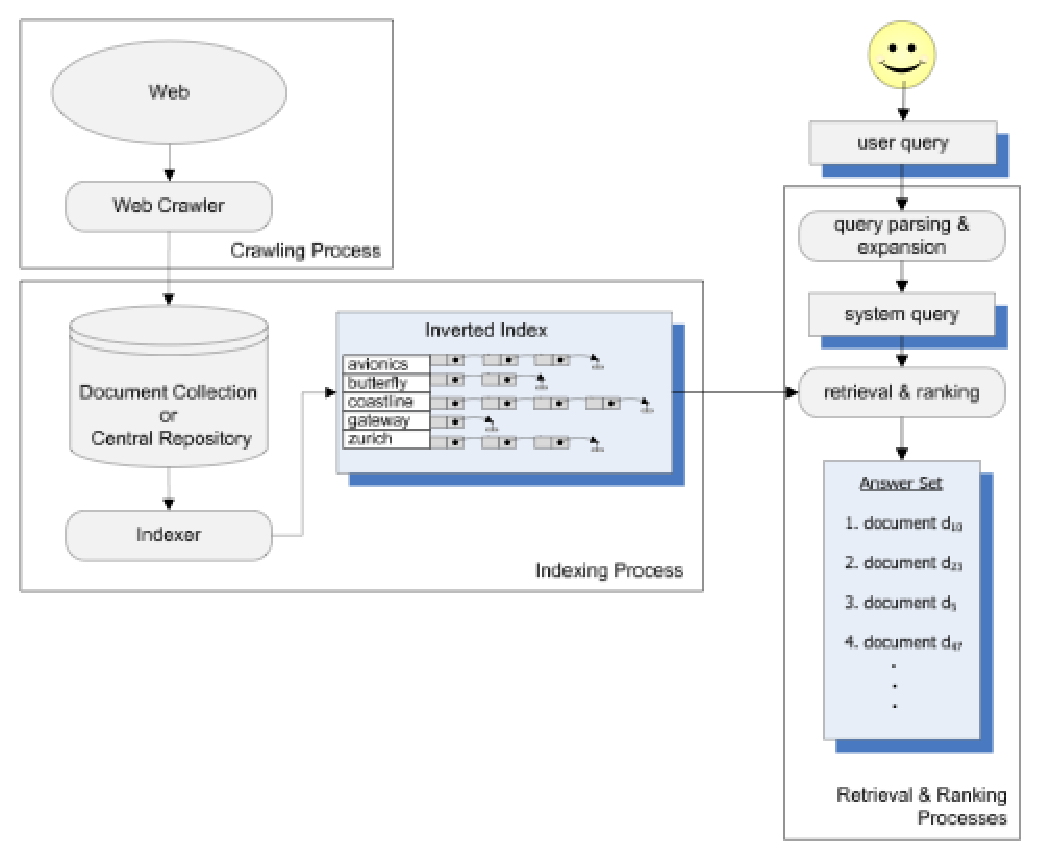
\includegraphics[width=1.0\textwidth]{fig/ir-architecture.eps}

	\legend{Fonte: \cite{mir2ed}}
\end{figure}

%\textbf{Explicação da figura.}
A figura \ref{fig:ir-architecture} apresenta a arquitetura de um sistema de recuperação de informação, o qual pode ser alterado para indexar e recuperar informação corporativa usando uma estrutura facetada sem alterações em sua arquitetura.

%\textbf{Ausência de coletor de documentos.}
Este trabalho adotou a coleção pública já pronta, sem a necessidade que um coletor (\textit{Web Crawler}) fosse implementado e usado. Assim, o primeiro componente implementado foi um indexador (\textit{indexer}).

%\textbf{Componente Indexador.}
O indexador automático (\textit{indexer}) é responsável por representar a coleção de documentos através de índices. Foram implementadas as seguintes estruturas de dados para representar ítens reconhecidos no conteúdo dos documentos: um arquivo invertido (\textit{inverted index}), estrutura padrão do Apache Lucene, para representar os termos; um \textit{gazetteer} para representar os termos geográficos; uma linha do tempo para representar as datas; e listas para representar atividades econômicas, documentos, pessoas, unidades organizacionais e patrimônio (equipamentos e \textit{softwares}).

%\textbf{Componente de interface de busca.}
O usuário de informação realiza sua busca através de uma interface com o usuário. Foi implementada uma interface com o usuário exclusivamente para testes eventuais do protótipo de sistema de recuperação de informação. Para uma execução mais rápida das 77 buscas, foi implementado um componente de processamento não assistido de consultas. Esse componente não faz parte de um sistema clássico de recuperação de informação e, portanto, não está presente na figura \ref{fig:ir-architecture}.

%\textbf{Componente Processador de Expressão de busca.}
O processador de expressão de busca (\textit{query parsing \& expansion}) é responsável por reconhecer as palavras-chaves informadas pelo usuário de informação e por reescrever a expressão de busca do usuário, incluindo ou retirando termos para aumentar a eficácia da recuperação. Neste componente foi implementado um método para reconhecer a faceta à qual pertence cada termo, produzindo uma reescrita mais elaborada. Em caso de expansão, exclusão ou alteração de termo, a operação ocorre exclusivamente dentro da faceta correspondente.

%\textbf{Componente de recuperação de informação.}
A expressão de busca final deve ser processada pelo componente de recuperação e ordenação (\textit{retrieval \& ranking}). O componente é responsável por recuperar os documentos supostamente de interesse e ordená-los em função de uma métrica de relevância. A métrica de relevância adotada é a \textit{term frequency-inverse document frequency} (TF-IDF), padrão no Apache Lucene, sem associar pesos diferentes para as facetas.



\subsection{Indexação automática da informação corporativa}
\label{prototipo-indexacao}

%\textbf{Tempo de indexação.}
A indexação automática da coleção pública consumiu um tempo total de 680856 milissegundos (ou 11,3476 minutos) em um computador com \textit{chipset} de 32 bits; processador Intel Core 2 Duo, P8400, com frequência de 2268 MHz; disco rígido de 160GiB, com 5400 rotações por minuto; memória principal de 4 GiB, frequência de 800 MHz; e sistema operacional Linux 32 bits.

%\textbf{Índices do SRI.}
O indexador automático representou a coleção por meio de oito índices, algo possível após a leitura técnica empreendida no capítulo anterior. O primeiro índice, um arquivo invertido, indexou todos as palavras presentes no conteúdo dos documentos. O segundo índice, um \textit{gazetteer}, indexou países, estados, territórios australianos, cidades, oceanos e mares, equipamentos urbanos e outras feições geográficas úteis, entre naturais, artificiais e cartográficas. Todas as referências geográficas indexadas estão presentes nas tabelas \ref{assuntosCSIROquery} e \ref{assuntosCSIROdocs}. O terceiro índice, uma linha do tempo, indexou as referências a anos encontradas no conteúdo dos documentos, utilizando-se de uma estratégia ingênua de associar qualquer palavra, ou \textit{token}, formada por quatro números como uma suposta referência a um ano. Os índices restantes, formados como listas ordenadas alfabeticamente, indexaram as referências às atividades econômicas, documentos, pessoas, unidades organizacionais e patrimônios da empresa.

%\textbf{Sem processamento de linguagem natural.}
Neste protótipo, nenhum índice dependeu do processamento de texto para interpretar as referências e aumentar sua precisão. Isto é, referências tais como "ano passado", "década anterior", "próximo a Sydney", "entre Sydney e Camberra" e outras são indexadas de maneira imprecisa, sem tratamento espaço-temporal do texto. Essa omissão não constitui uma recomendação para o projeto de um sistema de recuperação de informação, mas uma simples limitação do protótipo.

%\textbf{Link para a próxima seção.}
Na próxima seção são apresentadas as expressões de busca e de que forma ocorreu o processamento das expressões de busca para realizar a recuperação de informação da coleção pública.



\subsection{Processamento automático de consultas}
\label{prototipo-consultas}

%\textbf{Modelo de interação avaliado.}
Em uma parcela dos sistema de recuperação de informação, o usuário deve traduzir sua necessidade de informação em palavras-chaves na forma de uma expressão de busca. Dado um conjunto de palavras-chaves, o sistema de recuperação de informação deve converter as palavras-chaves em uma lista ordenada de documentos de interesse. É esse modelo de interação e de recuperação de informação corporativa que foi avaliado na trilha \textit{Enterprise} da \textit{Text Retrieval Conference} até o ano de 2008.

%\textbf{Explicação sobre a estratégia de busca facetada usando um local.}
Porém, no protótipo corporativo e facetado implementado nesta tese, termos fornecidos pelo usuário são convertidos em facetas antes de se executar a recuperação. Assim, não se busca por um termo ``victoria'' em documentos. Ao invés disso, se busca pela faceta Estado dentro dos documentos, usando a cadeia Melbourne, Victoria, Vic, Australia e Oceania como possíveis valores para a faceta, ou usando outros valores de outras facetas do renque.
Dessa forma, mesmo que Victoria não exista em qualquer documento, como a categoria Estado está presente, podem ser utilizados os estados das unidades organizacionais da empresa, os estados dos funcionários, dos projetos ou de outras entidades corporativas. Referências a Victoria são buscadas indiretamente.

%\textbf{Explicação sobre a estratégia de busca usando um nome de pessoa.}
Outro exemplo é o nome ``John''. Embora John seja um termo, o objeto de interesse pode ser a faceta cliente, faceta funcionário, ou a faceta Pessoa externa. Assim, são adotadas listas de funcionários, de clientes e de colaboradores, especialmente aquelas em que algum John exista. 

%\textbf{Implicações dessa estratégia de busca em outros modelos de interação.}
Essa estratégia também pode favorecer o \textit{browsing}  da coleção, em uma possível navegação facetada. Nesse modelo de interação com o usuário, critérios de ordenação são diferentes para cada expressão de busca, especialmente naquelas em que alguma categoria seja mais importante que as outras. Assim, Funcionários assumiriam ordem alfabética. Relatórios assumiriam ordem crescente de ano. Unidades organizacionais assumiriam ordem da mais importante para a menos importante, ou da mais próxima para a mais distante do usuário da informação. Porém, apenas a recuperação da informação facetada foi implementada no escopo dessa tese para buscar sua validação através da avaliação da trilha \textit{Enterprise}. Pois não há detalhes suficientes na trilha para avaliar diferentes critérios de ordenação e diferentes interfaces de usuário.

% Expressões de busca

%\textbf{Tabela original de 77 expressões de busca.}
A tabela \ref{tabQueriesOriginais} apresenta as 77 expressões de busca fornecidas juntamente com a coleção pública. Embora as narrativas, que explicam as expressões de busca, tenham sido estudadas no capítulo anterior, elas não foram adotadas na avaliação da recuperação. As 77 expressões de busca foram submetidas para um sistema de recuperação de informação, usando método de similaridade \textit{text frequency-inverse document frequency} (TF-IDF).

%\scriptsize
\begin{center}
%\begin{longtable}{p{4cm}|l|l|l|l}
\begin{longtable}{c|p{6cm}}
\caption[Expressões de busca originais da coleção pública]{Expressões de busca originais da coleção pública}
\label{tabQueriesOriginais}

\hline \textbf{Query} & \centering \textbf{Expressão de busca original} \\ \hline 
\endfirsthead

\multicolumn{2}{c}%
{{\bfseries \tablename\ \thetable{} -- continuação da página anterior}} \\
\hline \textbf{Query} &  \centering \textbf{Expressão de busca original} \\ \hline 
\endhead

\hline \multicolumn{2}{r}{{Continua na próxima página}} \\ \hline
\endfoot

%\hline % Retirada para incluir Fonte.
\endlastfoot




51 & weatherwall \\
52 & solve magazine \\
53 & selenium soil \\
54 & the heat is on \\
55 & case moth identification \\
56 & 12345+ \\
57 & fast instruments \\
58 & wood borer treatment \\
59 & vinelogic cd \\
60 & algae hydrogen powered cars \\
61 & wheel motor \\
62 & climate change hops \\
63 & vinegar bugs \\
64 & ant identification \\
65 & recruitment \\
66 & chilli paste preservatives \\
67 & sydney ocean temperatures \\
68 & sea level changes East Coast \\
69 & magnesium supplement \\
70 & information technology jobs \\
71 & termite wings \\
72 & biodegradable materials \\
73 & postdoctoral bioinformatics \\
74 & rene van berkel \\
75 & water conservation industry \\
76 & electric vehicles \\
77 & climate change \\
78 & pem micro fuel cells \\
79 & internship \\
80 & biodiversity \\
81 & artificial photosynthesis \\
82 & total wellbeing diet seafood \\
83 & contact scientist \\
84 & drought nsw \\
85 & water level property \\
86 & rabies test \\
87 & treated timber edible plants \\
88 & improving the built environment \\
89 & postdoctoral \\
90 & plant heavy metal binding proteins \\
91 & ultracapacitors \\
92 & cane toad photo \\
93 & annual report \\
94 & ants \\
95 & plant gene technology \\
96 & ocean floor map \\
97 & shipping container simulate \\
98 & insect identification \\
99 & training coordinator \\
100 & water food production \\
101 & trials weight loss \\
102 & nathers accurate \\
103 & forensic science workshop \\
104 & uranium reserves \\
105 & venture capital investment \\
106 & biodegradable plastic \\
107 & total wellbeing diet book 2 exercise \\
108 & millipede control \\
109 & employment aquaculture \\
110 & postdoctoral mathematics \\
111 & salinity wa \\
112 & mineral energy resources Australia \\
113 & sea levels \\
114 & millipedes \\
115 & hybrid cars \\
116 & friction coal crush \\
117 & freon climate change \\
118 & termite bait box \\
119 & melbourne events calendar \\
120 & bubbles ice image \\
121 & australia population \\
122 & images \\
123 & website feedback \\
124 & euclid eucalypts \\
125 & cervical cancer vaccination \\
126 & fish oil \\
127 & government funding \\


\hline
\hline \multicolumn{2}{l}{Fonte: Elaborada pelo autor.}

\end{longtable}
\end{center}
%\normalsize



%\textbf{Tabela modificada de queries.}
Em seguida, foram removidos os termos de facetas especiais e temporais das 77 expressões de busca, reescritas na coluna Base da tabela \ref{tabQueries}. Uma pré-consulta usando a expressão base forneceu suposto contexto espacial válido, ilustrado como um texto adicional da expressão de busca na coluna Espaço. A mesma pré-consulta forneceu suposto contexto temporal válido, ilustrado como um texto adicional da expressão de busca na coluna Tempo. E a mesma pré-consulta retornou a expressão base expandida (e/ou contraída), ilustrada como um texto adicional na coluna Alteração da tabela \ref{tabQueries}.








%\scriptsize
\begin{center}
%\begin{longtable}{p{4cm}|l|l|l|l}
\begin{longtable}{c|p{3cm}|c|c|p{3cm}}
\caption[Expressões de busca por informação facetada]{Expressões de busca por informação facetada. \\ \\ A expressão base é a menor parte da expressão original que não descaracterize a expressão original; as colunas Espaço e Tempo incluem parte especializada da expressão para as facetas Espaço e Tempo, respectivamente; a coluna Alteração apresenta expansões e contrações nas expressões de busca, isto é, termos que são incluídos e termos que são excluídos, \sout{rasurados como neste exemplo}, da expressão base.}
\label{tabQueries}

\hline \textbf{Query} & \centering \textbf{Base} & \textbf{Espaço} & \textbf{Tempo} &  \centering \textbf{Alteração} \\ \hline 
\endfirsthead

\multicolumn{5}{c}%
{{\bfseries \tablename\ \thetable{} -- continuação da página anterior}} \\
\hline \textbf{Query} & \centering \textbf{Base} & \textbf{Espaço} & \textbf{Tempo} &  \centering \textbf{Alteração} \\ \hline 
\endhead

\hline \multicolumn{5}{r}{{Continua na próxima página}} \\ \hline
\endfoot

%\hline % Retirada para incluir Fonte.
\endlastfoot


51 & weatherwall & melbourne &  &  \\ \hline
52 & solve magazine &  &  &  \\ \hline
53 & selenium soil & australia &  &  \\ \hline
54 & the heat is on &  & 2006 &  \\ \hline
55 & case moth identification &  &  &  \\ \hline
56 & 12345+ &  & 2006 &  \\ \hline
57 & FAST instruments &  &  &  \\ \hline
58 & wood borer treatment &  &  &  \\ \hline
59 & vinelogic cd &  & 2005 & \sout{cd} \\ \hline
60 & algae hydrogen powered cars &  &  &  \\ \hline
61 & wheel motor &  &  &  \\ \hline
62 & climate change hops &  & 2000-2009 &  \\ \hline
63 & vinegar bugs &  &  &  \\ \hline
64 & ant identification &  &  &  \\ \hline
65 & recruitment &  & 2007 & position \\ \hline
66 & chilli paste preservatives &  &  &  \\ \hline
67 & ocean temperatures & australia & 2000 &  \\ \hline
68 & sea level changes & australia & 2007 &  \\ \hline
69 & magnesium supplement &  &  &  \\ \hline
70 & information technology jobs &  & 2000-2009 &  \\ \hline
71 & termite wings &  &  &  \\ \hline
72 & biodegradable materials &  &  &  \\ \hline
73 & postdoctoral bioinformatics &  & 2007 & \sout{bioinformatics} position \\ \hline
74 & rene van berkel &  &  & \sout{rene van} contact \\ \hline
75 & water conservation industry &  & 2000-2009 &  \\ \hline
76 & electric vehicles &  &  &  \\ \hline
77 & climate change &  & 2000-2009 &  \\ \hline
78 & pem micro fuel cells &  &  &  \\ \hline
79 & internship &  & 2007 & position \\ \hline
80 & biodiversity &  &  &  \\ \hline
81 & artificial photosynthesis &  &  &  \\ \hline
82 & total wellbeing diet seafood &  & 2007 &  \\ \hline
83 & contact scientist &  &  &  \\ \hline
84 & drought & nsw & 1990-2009 &  \\ \hline
85 & water level property &  & 2000 &  \\ \hline
86 & rabies test &  &  &  \\ \hline
87 & treated timber edible plants &  &  &  \\ \hline
88 & improving the built environment &  &  &  \\ \hline
89 & postdoctoral &  & 2000-2009 & position \\ \hline
90 & plant heavy metal binding proteins &  &  &  \\ \hline
91 & ultracapacitors &  &  &  \\ \hline
92 & cane toad photo &  &  &  \\ \hline
93 & annual report &  & 2000-2009 &  \\ \hline
94 & ants &  &  &  \\ \hline
95 & plant gene technology &  & 2000-2009 &  \\ \hline
96 & ocean floor map &  & 2000-2009 &  \\ \hline
97 & shipping container simulate &  &  &  \\ \hline
98 & insect identification &  &  &  \\ \hline
99 & training coordinator &  & 2000-2009 & contact \\ \hline
100 & water food production &  & 2000 &  \\ \hline
101 & trials weight loss &  & 2007 &  \\ \hline
102 & nathers accurate &  & 2000-2009 &  \\ \hline
103 & forensic science workshop &  & 2007 &  \\ \hline
104 & uranium reserves &  & 2000 &  \\ \hline
105 & venture capital investment &  & 2000-2009 &  \\ \hline
106 & biodegradable plastic &  &  &  \\ \hline
107 & total wellbeing diet book 2 exercise &  & 2007 &  \\ \hline
108 & millipede control &  &  &  \\ \hline
109 & employment aquaculture &  & 2000-2009 &  \\ \hline
110 & postdoctoral mathematics &  & 2000-2009 & \sout{mathematics} position \\ \hline
111 & salinity & australia & 2000-2009 &  \\ \hline
112 & mineral energy resources & australia & 2000-2009 &  \\ \hline
113 & sea levels & australia & 2000-2009 &  \\ \hline
114 & millipedes &  &  &  \\ \hline
115 & hybrid cars &  &  &  \\ \hline
116 & friction coal crush &  &  &  \\ \hline
117 & freon climate change &  & 2000-2009 &  \\ \hline
118 & termite bait box &  &  &  \\ \hline
119 & events calendar & australia & 2000-2009 &  \\ \hline
120 & bubbles ice image &  &  &  \\ \hline
121 & population & australia & 2000-2009 &  \\ \hline
122 & images &  &  &  \\ \hline
123 & website feedback &  &  &  \\ \hline
124 & euclid eucalypts &  &  &  \\ \hline
125 & cervical cancer vaccination &  & 2000-2009 &  \\ \hline
126 & fish oil &  &  &  \\ \hline
127 & government funding &  & 2000-2009 &  \\ \hline




\hline
\hline \multicolumn{5}{l}{Fonte: Elaborada pelo autor.}

\end{longtable}
\end{center}
%\normalsize








%\textbf{Consultas executadas na avaliação.}
Uma primeira consulta usando a expressão base forneceu resultados da recuperação de informação corporativa. Uma segunda consulta usando a expressão base complementada com a expressão espacial foi executada. Uma terceira consulta usando a expressão base, complementada com as expressões espacial e temporal, foi executada em seguida. Finalmente, uma quarta consulta usando a expressão base com as alterações da coluna Alteração, complementada com as expressões espacial e temporal, recuperou a última lista de documentos para avaliação. Quando não houve atualização da expressão de busca nas colunas Espaço, Tempo e/ou Alteração, a mesma expressão de busca da etapa anterior foi utilizada, produzindo resultados idênticos àqueles obtidos na execução anterior.

%\textbf{Sumário para os resultados.}
Todos os resultados estão apresentados nas tabelas \ref{infAP} e \ref{infNDCG} na próxima seção, \ref{prototipo-resultados-publica}. Os resultados do segundo experimento são discutidos na seção \ref{prototipo-discussoes-publica}.


%Na indexação de documentos, posso então incluir os termos de indexação índice. No entanto, devo também incluir as facetas que sejam mais importantes para aquele documento. Em uma busca sobre o modelo, ao invés de de enviar uma busca por São Paulo, eu poderia mapear SP para estado e buscar por Estado, genérico. Todos os documentos que tratem Estado são retornados, sendo que a ordenação tratada geograficamente. Isso é viável?



















\subsection{Resultados do experimento sobre a coleção pública}
\label{prototipo-resultados-publica}

%\textbf{5 resultados e 2 métricas de desempenho.}
Os resultados das cinco execuções de processamento de consulta foram medidos usando Precisão Média (\textit{Average Precision} - AP), na tabela \ref{infAP}, e Ganho Acumulado Descontado Normalizado (\textit{Normalized Discounted Cumulative Gain}, NDCG), na tabela \ref{infNDCG}.

%\textbf{1a execução.}
A primeira execução de processamento de consulta deu-se usando a expressão de busca original, usando o método de similaridade TF-IDF e nenhum algoritmo que se beneficiava da organização facetada da informação. Os valores de AP e NDCG dessa primeira execução constituíram a base de comparação de desempenho das demais execuções do experimento.

%\textbf{2a execução.}
A segunda execução deu-se usando a expressão de busca base, excluídos termos de facetas espaciais e temporais. Essa execução também usou o método de similaridade TF-IDF e nenhum algoritmo que se beneficiava da organização facetada da informação. O valor de AP média foi 0,55\% superior ao da primeira execução. O valor de NDCG médio foi 0,50\% superior ao da primeira execução. 

%\textbf{Diferenças entre a 2a e 1a execução.}
Sete expressões de busca foram diferentes daquelas usadas na primeira execução. Em três delas houve aumento do desempenho considerando as duas métricas. Em três delas houve redução do desempenho considerando as duas métricas. Em uma das expressões de busca o desempenho melhorou pela métrica NDCG e piorou pela métrica AP.





%\scriptsize
\begin{center}
%\begin{longtable}{p{4cm}|l|l|l|l}
\begin{longtable}{c|r|r|r|r|r}
\caption[Resultado da métrica AP para experimentos sobre a coleção pública]{Resultado da métrica Precisão Média (\textit{Average Precision}, AP) para experimentos sobre a coleção pública. \\ \\ Os resultados são apresentados individualmente, por expressão de busca (\textit{query}), e agregados em uma média aritmética na última linha. As cinco colunas de resultados representam os resultados dos experimentos que usam 1) a expressão original; 2) a expressão base; 3) expressão base e faceta espacial; 4) expressão base e facetas espacial e temporal; 5) expressão base, facetas espacial e temporal, e expansões e contrações da expressão de busca.}
\label{infAP}

\hline \textbf{Query} & \textbf{infAP1} & \textbf{infAP2} & \textbf{infAP3}  & \textbf{infAP4}  & \textbf{infAP5}  \\ \hline 
\endfirsthead

\multicolumn{6}{c}%
{{\bfseries \tablename\ \thetable{} -- continuação da página anterior}} \\
\hline \textbf{Query} & \textbf{infAP1} & \textbf{infAP2} & \textbf{infAP3}  & \textbf{infAP4}  & \textbf{infAP5} \\ \hline 
\endhead

\hline \multicolumn{6}{r}{{Continua na próxima página}} \\ \hline
\endfoot

%\hline % Retirada para incluir Fonte.
\endlastfoot


52 & 0,4000 & 0,4000 & 0,4000 & 0,4000 & 0,4000 \\

53 & 0,2212 & 0,2212 & 0,4607 & 0,4607 & 0,4607 \\

54 & 0,0025 & 0,0025 & 0,0025 & 0,0077 & 0,0077 \\

56 & 0,2628 & 0,2628 & 0,2628 & 0,3353 & 0,3353 \\

57 & 0,3471 & 0,3471 & 0,3471 & 0,3471 & 0,3471 \\

58 & 0,3078 & 0,3078 & 0,3078 & 0,3078 & 0,3078 \\

59 & 0,5223 & 0,5223 & 0,5223 & 0,5741 & 0,7980 \\

60 & 0,3353 & 0,3353 & 0,3353 & 0,3353 & 0,3353 \\

61 & 0,8401 & 0,8401 & 0,8401 & 0,8401 & 0,8401 \\

62 & 0,2114 & 0,2114 & 0,2114 & 0,2105 & 0,2105 \\

63 & 0,0000 & 0,0000 & 0,0000 & 0,0000 & 0,0000 \\

64 & 0,6318 & 0,6318 & 0,6318 & 0,6318 & 0,6318 \\

65 & 0,0136 & 0,0136 & 0,0136 & 0,0137 & 0,0928 \\

67 & 0,0781 & 0,1496 & 0,1572 & 0,2714 & 0,2714 \\

68 & 0,1179 & 0,4745 & 0,4396 & 0,4441 & 0,4441 \\

69 & 0,0785 & 0,0785 & 0,0785 & 0,0785 & 0,0785 \\

70 & 0,0160 & 0,0160 & 0,0160 & 0,0161 & 0,0161 \\

71 & 0,1935 & 0,1935 & 0,1935 & 0,1935 & 0,1935 \\

72 & 0,6626 & 0,6626 & 0,6626 & 0,6626 & 0,6626 \\

73 & 0,0468 & 0,0468 & 0,0468 & 0,0431 & 0,0429 \\

75 & 0,3562 & 0,3562 & 0,3562 & 0,3559 & 0,3559 \\

76 & 0,4934 & 0,4934 & 0,4934 & 0,4934 & 0,4934 \\

77 & 0,5206 & 0,5206 & 0,5206 & 0,5206 & 0,5206 \\

79 & 0,0000 & 0,0000 & 0,0000 & 0,0000 & 0,0000 \\

80 & 0,3423 & 0,3423 & 0,3423 & 0,3423 & 0,3423 \\

82 & 0,4505 & 0,4505 & 0,4505 & 0,4714 & 0,4714 \\

83 & 0,1976 & 0,1976 & 0,1976 & 0,1976 & 0,1976 \\

84 & 0,1957 & 0,0801 & 0,1957 & 0,2390 & 0,2390 \\

85 & 0,0083 & 0,0083 & 0,0083 & 0,0140 & 0,0140 \\

86 & 0,5318 & 0,5318 & 0,5318 & 0,5318 & 0,5318 \\

87 & 0,1043 & 0,1043 & 0,1043 & 0,1043 & 0,1043 \\

88 & 0,1989 & 0,1989 & 0,1989 & 0,1989 & 0,1989 \\

89 & 0,1732 & 0,1732 & 0,1732 & 0,1732 & 0,1576 \\

90 & 0,0091 & 0,0091 & 0,0091 & 0,0091 & 0,0091 \\

93 & 0,3370 & 0,3370 & 0,3370 & 0,3369 & 0,3369 \\

94 & 0,4468 & 0,4468 & 0,4468 & 0,4468 & 0,4468 \\

95 & 0,4641 & 0,4641 & 0,4641 & 0,4629 & 0,4629 \\

96 & 0,5871 & 0,5871 & 0,5871 & 0,5874 & 0,5874 \\

97 & 0,0229 & 0,0229 & 0,0229 & 0,0229 & 0,0229 \\

98 & 0,1502 & 0,1502 & 0,1502 & 0,1502 & 0,1502 \\

99 & 0,0366 & 0,0366 & 0,0366 & 0,0363 & 0,0445 \\

100 & 0,1009 & 0,1009 & 0,1009 & 0,1055 & 0,1055 \\

102 & 0,6097 & 0,6097 & 0,6097 & 0,6013 & 0,6013 \\

105 & 0,1563 & 0,1563 & 0,1563 & 0,1522 & 0,1522 \\

106 & 0,2077 & 0,2077 & 0,2077 & 0,2077 & 0,2077 \\

109 & 0,1826 & 0,1826 & 0,1826 & 0,1796 & 0,1796 \\

110 & 0,1363 & 0,1363 & 0,1363 & 0,1331 & 0,5555 \\

111 & 0,3021 & 0,2288 & 0,2801 & 0,2779 & 0,2779 \\

112 & 0,2247 & 0,2194 & 0,2247 & 0,2245 & 0,2245 \\

113 & 0,2758 & 0,2758 & 0,3177 & 0,3218 & 0,3218 \\

114 & 0,2619 & 0,2619 & 0,2619 & 0,2619 & 0,2619 \\

115 & 0,7827 & 0,7827 & 0,7827 & 0,7827 & 0,7827 \\

117 & 0,0530 & 0,0530 & 0,0530 & 0,0531 & 0,0531 \\

118 & 0,6638 & 0,6638 & 0,6638 & 0,6638 & 0,6638 \\

119 & 0,0116 & 0,0120 & 0,0161 & 0,0160 & 0,0160 \\

120 & 0,6485 & 0,6485 & 0,6485 & 0,6485 & 0,6485 \\

121 & 0,2243 & 0,0857 & 0,2243 & 0,2223 & 0,2223 \\

122 & 0,0000 & 0,0000 & 0,0000 & 0,0000 & 0,0000 \\

123 & 0,0760 & 0,0760 & 0,0760 & 0,0760 & 0,0760 \\

125 & 0,5787 & 0,5787 & 0,5787 & 0,5720 & 0,5720 \\

126 & 0,0751 & 0,0751 & 0,0751 & 0,0751 & 0,0751 \\

127 & 0,3323 & 0,3323 & 0,3323 & 0,3373 & 0,3373 \\

Média & 0,2713 & 0,2728 & 0,2818 & 0,2868 & 0,2984 \\



\hline
\hline \multicolumn{6}{l}{Fonte: Elaborada pelo autor.}

\end{longtable}
\end{center}
%\normalsize





%\textbf{3a execução.}
A terceira execução deu-se usando a expressão de busca base, complementada com algum termo de faceta espacial caso algum termo tenha sido recomendado na pré-consulta. Essa execução fez uso de um algoritmo que se beneficiava da organização facetada da informação, escolhendo o foco geográfico mais adequado para cada expressão de busca. O valor de AP média foi 3,30\% superior ao da execução anterior. O valor de NDCG médio foi 2,48\% superior ao da execução anterior. 

%\textbf{Diferenças entre 3a e 2a execução.}
Nove expressões de busca foram diferentes daquelas usadas na segunda execução. Em oito delas houve aumento do desempenho considerando as duas métricas. Em uma das expressões de busca houve redução do desempenho considerando as duas métricas.

%\textbf{4a execução.}
A quarta execução deu-se usando a expressão de busca base e da faceta espacial, complementada com algum termo de faceta temporal caso algum termo tenha sido recomendado na pré-consulta. Essa execução fez uso de um algoritmo que escolhia o foco temporal mais adequado para cada expressão de busca. O valor de AP média foi 1,77\% superior ao da execução anterior. O valor de NDCG médio foi 1,61\% superior ao da execução anterior. 

%\textbf{Diferenças entre 4a e 3a execução.}
Trinta e sete expressões de busca foram diferentes daquelas usadas na terceira execução. Dessas, apenas 31 buscas foram avaliadas na quarta execução. Em 11 delas houve aumento do desempenho considerando as duas métricas. Em nove delas houve redução do desempenho considerando as duas métricas. Em cinco das expressões de busca o desempenho melhorou pela métrica NDCG e piorou pela métrica AP. Ao contrário, em quatro das expressões de busca o desempenho piorou pela métrica NDCG e melhorou pela métrica AP. Finalmente, em duas das expressões de busca o desempenho não sofreu alteração quando comparado ao desempenho da execução anterior.

%\textbf{5a execução.}
A quinta execução deu-se usando a expressão de busca base, da faceta espacial e da faceta temporal, alteradas pela adição ou exclusão de termos indicados na pré-consulta. Essa execução fez uso de um algoritmo que inclui ou remove termos da expressão de busca, escolhendo a melhor representação para cada faceta mobilizada pelo usuário da informação na elaboração da expressão de busca. O valor de AP média foi 4,04\% superior ao da execução anterior. O valor de NDCG médio foi 1,52\% superior ao da execução anterior.

%\textbf{Diferenças entre a 5a e a 4a execução.}
Oito expressões de busca foram diferentes daquelas usadas na quarta execução. Dessas, apenas seis buscas foram avaliadas na quinta execução. Em três delas houve aumento do desempenho considerando as duas métricas. Em uma delas houve redução do desempenho considerando as duas métricas. Em uma das expressões de busca o desempenho melhorou pela métrica NDCG e piorou pela métrica AP. Ao contrário, em uma das expressões de busca o desempenho piorou pela métrica NDCG e melhorou pela métrica AP.









%\scriptsize
\begin{center}
%\begin{longtable}{p{4cm}|l|l|l|l}
\begin{longtable}{c|r|r|r|r|r}
\caption[Resultado da métrica NDCG para experimentos sobre a coleção pública]{Resultado da métrica Ganho Acumulado Descontado Normalizado (\textit{Normalized Discounted Cumulative Gain}, NDCG) para experimentos sobre a coleção pública. \\ \\Os resultados são apresentados individualmente, por expressão de busca (\textit{query}), e agregados em uma média aritmética na última linha. As cinco colunas de resultados representam os resultados dos experimentos que usam 1) a expressão original; 2) a expressão base; 3) expressão base e faceta espacial; 4) expressão base e facetas espacial e temporal; 5) expressão base, facetas espacial e temporal, e expansões e contrações da expressão de busca.}
\label{infNDCG}

\hline \textbf{Query} & \textbf{infNDCG1} & \textbf{infNDCG2} & \textbf{infNDCG3}  & \textbf{infNDCG4}  & \textbf{infNDCG5}  \\ \hline 
\endfirsthead

\multicolumn{6}{c}%
{{\bfseries \tablename\ \thetable{} -- continuação da página anterior}} \\
\hline \textbf{Query} & \textbf{infNDCG1} & \textbf{infNDCG2} & \textbf{infNDCG3}  & \textbf{infNDCG4}  & \textbf{infNDCG5} \\ \hline 
\endhead

\hline \multicolumn{6}{r}{{Continua na próxima página}} \\ \hline
\endfoot

%\hline % Retirada para incluir Fonte.
\endlastfoot


52 & 0,4841 & 0,4841 & 0,4841 & 0,4841 & 0,4841 \\

53 & 0,4947 & 0,4947 & 0,7388 & 0,7388 & 0,7388 \\

54 & 0,0600 & 0,0600 & 0,0600 & 0,1706 & 0,1706 \\

56 & 0,5495 & 0,5495 & 0,5495 & 0,5941 & 0,5941 \\

57 & 0,5100 & 0,5100 & 0,5100 & 0,5100 & 0,5100 \\

58 & 0,4343 & 0,4343 & 0,4343 & 0,4343 & 0,4343 \\

59 & 0,6682 & 0,6682 & 0,6682 & 0,8778 & 0,9557 \\

60 & 0,5459 & 0,5459 & 0,5459 & 0,5459 & 0,5459 \\

61 & 0,7653 & 0,7653 & 0,7653 & 0,7653 & 0,7653 \\

62 & 0,4775 & 0,4775 & 0,4775 & 0,4771 & 0,4771 \\

63 & 0,0000 & 0,0000 & 0,0000 & 0,0000 & 0,0000 \\

64 & 0,6788 & 0,6788 & 0,6788 & 0,6788 & 0,6788 \\

65 & 0,1111 & 0,1111 & 0,1111 & 0,1110 & 0,2565 \\

67 & 0,3646 & 0,5642 & 0,6247 & 0,6436 & 0,6436 \\

68 & 0,3469 & 0,7310 & 0,6808 & 0,6739 & 0,6739 \\

69 & 0,4234 & 0,4234 & 0,4234 & 0,4234 & 0,4234 \\

70 & 0,2525 & 0,2525 & 0,2525 & 0,2425 & 0,2425 \\

71 & 0,6317 & 0,6317 & 0,6317 & 0,6317 & 0,6317 \\

72 & 0,7731 & 0,7731 & 0,7731 & 0,7731 & 0,7731 \\

73 & 0,3514 & 0,3514 & 0,3514 & 0,3612 & 0,3709 \\

75 & 0,6565 & 0,6565 & 0,6565 & 0,6579 & 0,6579 \\

76 & 0,7212 & 0,7212 & 0,7212 & 0,7212 & 0,7212 \\

77 & 0,4966 & 0,4966 & 0,4966 & 0,4966 & 0,4966 \\

79 & 0,0000 & 0,0000 & 0,0000 & 0,0000 & 0,0000 \\

80 & 0,4752 & 0,4752 & 0,4752 & 0,4752 & 0,4752 \\

82 & 0,7078 & 0,7078 & 0,7078 & 0,7076 & 0,7076 \\

83 & 0,4432 & 0,4432 & 0,4432 & 0,4432 & 0,4432 \\

84 & 0,5973 & 0,4140 & 0,5973 & 0,6154 & 0,6154 \\

85 & 0,2196 & 0,2196 & 0,2196 & 0,2512 & 0,2512 \\

86 & 0,5400 & 0,5400 & 0,5400 & 0,5400 & 0,5400 \\

87 & 0,4315 & 0,4315 & 0,4315 & 0,4315 & 0,4315 \\

88 & 0,4737 & 0,4737 & 0,4737 & 0,4737 & 0,4737 \\

89 & 0,3363 & 0,3363 & 0,3363 & 0,3363 & 0,3303 \\

90 & 0,2610 & 0,2610 & 0,2610 & 0,2610 & 0,2610 \\

93 & 0,6298 & 0,6298 & 0,6298 & 0,6292 & 0,6292 \\

94 & 0,6969 & 0,6969 & 0,6969 & 0,6969 & 0,6969 \\

95 & 0,5572 & 0,5572 & 0,5572 & 0,5527 & 0,5527 \\

96 & 0,5936 & 0,5936 & 0,5936 & 0,5932 & 0,5932 \\

97 & 0,0796 & 0,0796 & 0,0796 & 0,0796 & 0,0796 \\

98 & 0,5124 & 0,5124 & 0,5124 & 0,5124 & 0,5124 \\

99 & 0,2374 & 0,2374 & 0,2374 & 0,2361 & 0,2311 \\

100 & 0,3787 & 0,3787 & 0,3787 & 0,4166 & 0,4166 \\

102 & 0,5785 & 0,5785 & 0,5785 & 0,5742 & 0,5742 \\

105 & 0,4935 & 0,4935 & 0,4935 & 0,4985 & 0,4985 \\

106 & 0,5516 & 0,5516 & 0,5516 & 0,5516 & 0,5516 \\

109 & 0,4759 & 0,4759 & 0,4759 & 0,4760 & 0,4760 \\

110 & 0,5272 & 0,5272 & 0,5272 & 0,5307 & 0,7828 \\

111 & 0,5136 & 0,5162 & 0,5602 & 0,5595 & 0,5595 \\

112 & 0,6069 & 0,5971 & 0,6069 & 0,6033 & 0,6033 \\

113 & 0,6432 & 0,6432 & 0,6447 & 0,6632 & 0,6632 \\

114 & 0,4254 & 0,4254 & 0,4254 & 0,4254 & 0,4254 \\

115 & 1,0044 & 1,0044 & 1,0044 & 1,0044 & 1,0044 \\

117 & 0,5013 & 0,5013 & 0,5013 & 0,5014 & 0,5014 \\

118 & 0,8274 & 0,8274 & 0,8274 & 0,8274 & 0,8274 \\

119 & 0,2337 & 0,2380 & 0,2587 & 0,2545 & 0,2545 \\

120 & 0,7456 & 0,7456 & 0,7456 & 0,7456 & 0,7456 \\

121 & 0,6201 & 0,3739 & 0,6201 & 0,6160 & 0,6160 \\

122 & 0,0000 & 0,0000 & 0,0000 & 0,0000 & 0,0000 \\

123 & 0,1909 & 0,1909 & 0,1909 & 0,1909 & 0,1909 \\

125 & 0,6543 & 0,6543 & 0,6543 & 0,6507 & 0,6507 \\

126 & 0,4232 & 0,4232 & 0,4232 & 0,4232 & 0,4232 \\

127 & 0,5743 & 0,5743 & 0,5743 & 0,5767 & 0,5767 \\

Média & 0,4768 & 0,4792 & 0,4911 & 0,4990 & 0,5066 \\





\hline
\hline \multicolumn{6}{l}{Fonte: Elaborada pelo autor.}

\end{longtable}
\end{center}
%\normalsize








%\textbf{Link para a próxima seção.}
As discussões sobre os resultados do experimento sobre a coleção pública são apresentadas na próxima seção, \ref{prototipo-discussoes-publica}.






\subsection{Discussões de resultados sobre a coleção pública}
\label{prototipo-discussoes-publica}

%\textbf{Introdução da seção.}
A seção \ref{prototipo-resultados-publica} apresentou os resultados empíricos da avaliação de um protótipo de sistema de recuperação de informação corporativa facetada usando os princípios e métricas da trilha \textit{Enterprise} da \textit{Text Retrieval Conference}. 

%\textbf{5 execuções, 2 métricas, apresentação da tabela de comparação com outros trabalhos da trilha Enterprise.}
Os resultados das cinco execuções de processamento de consulta foram medidos usando Precisão Média (\textit{Average Precision} - AP), na tabela \ref{infAP}, e Ganho Acumulado Descontado Normalizado (\textit{Normalized Discounted Cumulative Gain}, NDCG), na tabela \ref{infNDCG}. Os valores médios finais podem ser comparados com os valores alcançados por participantes da trilha \textit{Enterprise} na tabela \ref{tabDesempenhoFacetada}. Os resultados atendem ao objetivo de avaliar a eficiência da indexação e da recuperação de documentos da coleção corporativa de referência.








%\scriptsize
\begin{center}
%\begin{longtable}{p{4cm}|l|l|l|l}
\begin{longtable}{p{11cm}|c|c}
\caption[Desempenho da recuperação de informação facetada]{Desempenho da recuperação de informação facetada. \\ \\ Os resultados em negrito foram obtidos nesta tese. Os demais são resultados dos grupos que participaram da trilha \textit{Enterprise} da \textit{Text Retrieval Conference}, edição de 2008. Todos os resultados estão ordenados da maior precisão média para a menor precisão média.}
\label{tabDesempenhoFacetada}

\hline \centering \textbf{Origem do experimento} & infAP & infNDCG \\ \hline 
\endfirsthead

\multicolumn{3}{c}%
{{\bfseries \tablename\ \thetable{} -- continuação da página anterior}} \\
\hline \centering \textbf{Origem do experimento} & infAP & infNDCG \\ \hline 
\endhead

\hline \multicolumn{3}{r}{{Continua na próxima página}} \\ \hline
\endfoot

%\hline % Retirada para incluir Fonte.
\endlastfoot



UGlasgow  & 0,3891 & 0,5660 \\
CAS & 0,3760 & 0,5393 \\
Tsinghua & 0,3612 & 0,5578 \\
UAmsterdam  & 0,3306 & 0,4909 \\
UC-London & 0,3246 & 0,5175 \\
Fudan & 0,3204 & 0,4985 \\
UAvignon  & 0,3191 & 0,5078 \\
UArkansas  & 0,3024 & 0,4838 \\
NUI-Galway & 0,3018 & 0,4791 \\
\textbf{Ex5. Expressão Base+Espaço+Tempo com Expansão} & \textbf{0,2984} & \textbf{0,5066} \\
RMIT & 0,2975 & 0,5045 \\
\textbf{Ex4. Expressão Base+Espaço+Tempo} & \textbf{0,2868} & \textbf{0,4990} \\
\textbf{Ex3. Expressão Base+Espaço} & \textbf{0,2818} & \textbf{0,4911} \\
\textbf{Ex2. Expressão Base (TF-IDF)} & \textbf{0,2728} & \textbf{0,4792} \\
\textbf{Ex1. Original (TF-IDF)} & \textbf{0,2713} & \textbf{0,4768} \\
Sebir & 0,2252 & 0,4035 \\
BUPT & 0,2216 & 0,4046 \\
INRIA & 0,1879 & 0,3785 \\
SPSU & 0,1300 & 0,3057 \\




\hline
\hline \multicolumn{3}{l}{Fonte: Elaborada pelo autor.}

\end{longtable}
\end{center}
%\normalsize



%\textbf{Discussão sobre a 1a execução.}
A primeira execução (Ex1) serviu como referência para as outras quatro execuções. A primeira usou as expressões originais da trilha e a indexação não se beneficiou da organização facetada da informação e do conhecimento construído acerca do domínio corporativo. Adotando exclusivamente o modelo de similaridade TF-IDF, seu desempenho foi superior àquele obtido em alguns trabalhos da literatura, como se observa na tabela \ref{tabDesempenhoFacetada}. Isso encontra explicação no propósito da avaliação de Cranfield: descobrir métodos eficientes empiricamente pela comparação do seu desempenho. Assim, todos os experimentos, com alto ou baixo desempenho, são úteis para avançar o conhecimento sobre recuperação de informação.

%\textbf{Discussão sobre a 2a execução.}
Ainda sem adotar recursos do domínio corporativo, a segunda execução (Ex2) fez uso de expressões de busca simplificadas. Nela, as expressões não continham referências geográficas e temporais. Ao observar um aumento do desempenho da recuperação de informação, alguns trabalhos da literatura questionam se as facetas geográficas e temporais são realmente úteis. De fato, o que esses resultados parecem indicar é que a escolha incorreta do escopo geográfico e temporal, por parte do autor da expressão de busca, pode limitar a busca desnecessariamente e causar prejuízo ao processo de recuperação de informação.

%\textbf{Diferenças entre as execuções 3, 4 e 5 e as duas primeiras.}
Por outro lado, as execuções 3, 4 e 5 se beneficiaram de características do domínio corporativo, reconhecidas a partir do trabalho empreendido no capítulo \ref{analiseDominio}, e da organização facetada da informação corporativa. O aumento do desempenho médio das consultas em cada uma das três execuções deu-se pelo aumento significativo do desempenho de algumas poucas consultas. Na execução 3, por exemplo, 10,39\% das buscas foram responsáveis por todo o aumento de desempenho do experimento. Na execução 4 houve uma participação maior: 25,97\%. Finalmente, na execução 5, apenas 5,19\% das buscas foram responsáveis pelo maior aumento de desempenho registrado no experimento sobre a coleção pública.

%\textbf{Discussão da 3a execução.}
A terceira execução (Ex3) passou a conter referências geográficas na expressão de busca. Nela, o desempenho da recuperação aumentou ainda mais. Isso nos permite formular uma hipótese para o baixo desempenho de modelos espaciais em sistemas de recuperação de informação geográfica, quando comparados ao modelo TF-IDF. Os modelos mentais espaciais de autores de documentos e de expressões de busca parecem ser diferentes. Logo, georreferenciar as mensagens não é a solução final. Por outro lado, desambiguar e ajustar a precisão espacial das referências geográficas parece ser uma direção promissora, pois foi exatamente a abordagem adotada neste experimento.

%\textbf{Discussão da 4a execução.}
A quarta execução (Ex4), por sua vez, passou a conter referências temporais e geográficas na expressão de busca. Novamente, o desempenho da recuperação aumentou. Porém, não é possível supor que o modelo mental de tempo seja diferente entre autores de documento e de expressões de busca. Ao invés disso, mesmo que facetas temporais não sejam mobilizadas por usuários da informação, o sistema de recuperação de informação pode promover uma interface com o usuário que suporte o filtro e o \textit{ranking} de resultados, tornando mais eficaz o acesso à informação.

%\textbf{Discussão da 5a execução.}
A quinta execução (Ex5), finalmente, passou a conter referências mais apropriadas para cada faceta mobilizada na expressão base. O desempenho medido em Precisão Média chegou a aumentar em 4,04\%. Não é novidade que a escolha apropriada das palavras-chaves para compor a expressão de busca favorece a recuperação. No entanto, técnicas de expansão e contração de expressões de busca precisam reconhecer quais alterações são mais apropriadas. Identificar quais facetas, ao invés de termos, devam sofrer expansão ou contração parece promissor e mais simples.

%\textbf{Limitações dos resultados da tabela.}
Os resultados de todos os trabalhos apresentados na tabela \ref{tabDesempenhoFacetada} não foram completamente validados pelos profissionais de informação da CSIRO. Por isso, os resultados devem ser usados com cautela para o projeto de sistemas de recuperação de informação corporativa, mesmo que exclusivamente destinados para a CSIRO. O mesmo se aplica aos resultados deste experimento sobre a coleção pública.

%\textbf{Limitação das estratégias adotadas em experimentos da trilha Enterprise.}
Alguns dos experimentos realizados no âmbito da trilha \textit{Enterprise} se beneficiam de certas características que não são próprias do domínio corporativo. Provavelmente, algumas delas não são próprias nem mesmo da informação da CSIRO, tendo em vista que a coleção de referência apresenta o viés de possuir apenas páginas \textit{Web} públicas do \textit{site} da empresa. Adicionalmente, toda empresa é única e pode possuir características que sejam difíceis de encontrar em outras empresas. A CSIRO, especificamente, é um exemplar ainda mais incomum dentro do domínio corporativo, por sua atividade ser pesquisa científica, contar com profissionais de elevado nível de especialização e com nomes sempre presentes na imprensa e na \textit{Web}, ter grande capilaridade geográfica e ser proprietária de um grande volume de informação pública.

%\textbf{Discussão sobre trabalhos da trilha Enterprise - usando Wikipedia.}
Por exemplo, trabalhos como de \citeonline{he2008}, \citeonline{shen2008} e \citeonline{peng2008} fizeram uso de fontes externas como a Wikipedia para produzir expansão de expressões de busca. Isso parece útil e adequado para uma coleção composta de documentos de divulgação científica da CSIRO, com temas científicos diversos. No entanto, não se aplica a uma coleção mais homogênea, de empresa menor, constituída por documentos de comunicação empresarial interna. 

%\textbf{Discussão sobre trabalhos da trilha Enterprise - usando fontes de evidências sociais.}
Outros trabalhos, tais como \citeonline{balog2008} e \citeonline{cummins2008} combinaram a busca por especialistas e a busca por documentos. Certamente a estratégia foi útil para o caso CSIRO, especialmente se combinada com fontes externas de evidência. Trata-se de uma empresa de pesquisa científica, a maior da Austrália. Seus especialistas são doutores reconhecidos pela comunidade científica em todo o mundo em temas como melhoramento genético, oceanografia, controle de pragas, climatologia e outros. Todos aplicados às necessidades da região onde a Austrália se localiza, o que inclui países e continentes próximos. No entanto, a estratégia parece pouco apropriada a empresas onde não existam profissionais tão renomados, destacados e presentes em jornais, revistas e buscadores \textit{Web}.

%\textbf{Discussão sobre trabalhos da trilha Enterprise - usando o hipertexto.}
Também, trabalhos como \citeonline{xue2008} e \citeonline{zhu2008} se aproveitaram do fato de documentos da coleção serem da face \textit{Web} pública da CSIRO. Trata-se de uma estratégia que se beneficia da estrutura hipertextual, das ligações de entrada (\textit{inlinks}) e de saída (\textit{outlinks}) dos documentos, dos textos de ligação e de métodos de ordenação eficientes para a \textit{Web} como o \textit{PageRank}. Como a coleção de referência é corporativa, mas também é um subconjunto da Web, é natural adotar tal estratégia. Porém, o mesmo sucesso não ocorre na outra face da CSIRO, onde certamente existem documentos em outros formatos, sem hipertexto, sem ligações explícitas entre documentos, sem comandos de marcação da linguagem HTML.

%\textbf{Discussão sobre trabalhos da trilha Enterprise - usando frase ao invés de documento.}
Um último exemplo é o trabalho de \citeonline{sanjuan2008} que adotou seu método destinado a um sistema de resposta automática. O método aborda a informação com granularidade diferente, recuperando trechos do conteúdo dos documentos (frases e partes de frases), ao invés dos documentos. Certamente essa estratégia é promissora para o domínio corporativo e pode se beneficiar da organização facetada da informação corporativa. Por outro lado, a direção contrária de granularidade também é possível, considerando blocos de documentos, repositórios, tipos de documentos e outros conjuntos maiores. É provável que tipologia de documentos, estudos de gêneros textuais, métodos de bancos de dados estruturados e de dados ligados favoreçam de forma diferenciada as várias empresas que funcionam dentro de cada grande empresa.

%\textbf{Link para próximo capítulo}
No próximo capítulo, \ref{conclusao}, são apontadas conclusões, limitações deste trabalho e algumas direções de trabalho futuro.



%======================================================







% INÍCIO DAS TABELAS ANTIGAS - COMENTADO
\begin{comment}

%\scriptsize
\begin{center}
%\begin{longtable}{p{4cm}|l|l|l|l}
\begin{longtable}{c|r|r}
\caption[trec1]{trec1}
\label{trec1}

\hline \textbf{Expressão de busca} & \textbf{infAP} & \textbf{infNDCG} \\ \hline 
\endfirsthead

\multicolumn{3}{c}%
{{\bfseries \tablename\ \thetable{} -- continuação da página anterior}} \\
\hline \textbf{Busca} & \textbf{infAP} & \textbf{infNDCG} \\ \hline 
\endhead

\hline \multicolumn{3}{r}{{Continua na próxima página}} \\ \hline
\endfoot

%\hline % Retirada para incluir Fonte.
\endlastfoot

52 & 0,4000 & 0,4841 \\

53 & 0,2212 & 0,4947 \\

54 & 0,0025 & 0,0600 \\

56 & 0,2628 & 0,5495 \\

57 & 0,3471 & 0,5100 \\

58 & 0,3078 & 0,4343 \\

59 & 0,5223 & 0,6682 \\

60 & 0,3353 & 0,5459 \\

61 & 0,8401 & 0,7653 \\

62 & 0,2114 & 0,4775 \\

63 & 0,0000 & 0,0000 \\

64 & 0,6318 & 0,6788 \\

65 & 0,0136 & 0,1111 \\

67 & 0,0781 & 0,3646 \\

68 & 0,1179 & 0,3469 \\

69 & 0,0785 & 0,4234 \\

70 & 0,0160 & 0,2525 \\

71 & 0,1935 & 0,6317 \\

72 & 0,6626 & 0,7731 \\

73 & 0,0468 & 0,3514 \\

75 & 0,3562 & 0,6565 \\

76 & 0,4934 & 0,7212 \\

77 & 0,5206 & 0,4966 \\

79 & 0,0000 & 0,0000 \\

80 & 0,3423 & 0,4752 \\

82 & 0,4505 & 0,7078 \\

83 & 0,1976 & 0,4432 \\

84 & 0,1957 & 0,5973 \\

85 & 0,0083 & 0,2196 \\

86 & 0,5318 & 0,5400 \\

87 & 0,1043 & 0,4315 \\

88 & 0,1989 & 0,4737 \\

89 & 0,1732 & 0,3363 \\

90 & 0,0091 & 0,2610 \\

93 & 0,3370 & 0,6298 \\

94 & 0,4468 & 0,6969 \\

95 & 0,4641 & 0,5572 \\

96 & 0,5871 & 0,5936 \\

97 & 0,0229 & 0,0796 \\

98 & 0,1502 & 0,5124 \\

99 & 0,0366 & 0,2374 \\

100 & 0,1009 & 0,3787 \\

102 & 0,6097 & 0,5785 \\

105 & 0,1563 & 0,4935 \\

106 & 0,2077 & 0,5516 \\

109 & 0,1826 & 0,4759 \\

110 & 0,1363 & 0,5272 \\

111 & 0,3021 & 0,5136 \\

112 & 0,2247 & 0,6069 \\

113 & 0,2758 & 0,6432 \\

114 & 0,2619 & 0,4254 \\

115 & 0,7827 & 1,0044 \\

117 & 0,0530 & 0,5013 \\

118 & 0,6638 & 0,8274 \\

119 & 0,0116 & 0,2337 \\

120 & 0,6485 & 0,7456 \\

121 & 0,2243 & 0,6201 \\

122 & 0,0000 & 0,0000 \\

123 & 0,0760 & 0,1909 \\

125 & 0,5787 & 0,6543 \\

126 & 0,0751 & 0,4232 \\

127 & 0,3323 & 0,5743 \\

Todas & 0,2713 & 0,4768 \\


\hline
\hline \multicolumn{3}{l}{Fonte: Elaborada pelo autor.}

\end{longtable}
\end{center}
%\normalsize





%\scriptsize
\begin{center}
%\begin{longtable}{p{4cm}|l|l|l|l}
\begin{longtable}{c|r|r}
\caption[trec2]{trec2}
\label{trec1}

\hline \textbf{Expressão de busca} & \textbf{infAP} & \textbf{infNDCG} \\ \hline 
\endfirsthead

\multicolumn{3}{c}%
{{\bfseries \tablename\ \thetable{} -- continuação da página anterior}} \\
\hline \textbf{Busca} & \textbf{infAP} & \textbf{infNDCG} \\ \hline 
\endhead

\hline \multicolumn{3}{r}{{Continua na próxima página}} \\ \hline
\endfoot

%\hline % Retirada para incluir Fonte.
\endlastfoot


52 & 0,4000 & 0,4841 \\

53 & 0,2212 & 0,4947 \\

54 & 0,0025 & 0,0600 \\

56 & 0,2628 & 0,5495 \\

57 & 0,3471 & 0,5100 \\

58 & 0,3078 & 0,4343 \\

59 & 0,5223 & 0,6682 \\

60 & 0,3353 & 0,5459 \\

61 & 0,8401 & 0,7653 \\

62 & 0,2114 & 0,4775 \\

63 & 0,0000 & 0,0000 \\

64 & 0,6318 & 0,6788 \\

65 & 0,0136 & 0,1111 \\

67 & 0,1496 & 0,5642 \\

68 & 0,4745 & 0,7310 \\

69 & 0,0785 & 0,4234 \\

70 & 0,0160 & 0,2525 \\

71 & 0,1935 & 0,6317 \\

72 & 0,6626 & 0,7731 \\

73 & 0,0468 & 0,3514 \\

75 & 0,3562 & 0,6565 \\

76 & 0,4934 & 0,7212 \\

77 & 0,5206 & 0,4966 \\

79 & 0,0000 & 0,0000 \\

80 & 0,3423 & 0,4752 \\

82 & 0,4505 & 0,7078 \\

83 & 0,1976 & 0,4432 \\

84 & 0,0801 & 0,4140 \\

85 & 0,0083 & 0,2196 \\

86 & 0,5318 & 0,5400 \\

87 & 0,1043 & 0,4315 \\

88 & 0,1989 & 0,4737 \\

89 & 0,1732 & 0,3363 \\

90 & 0,0091 & 0,2610 \\

93 & 0,3370 & 0,6298 \\

94 & 0,4468 & 0,6969 \\

95 & 0,4641 & 0,5572 \\

96 & 0,5871 & 0,5936 \\

97 & 0,0229 & 0,0796 \\

98 & 0,1502 & 0,5124 \\

99 & 0,0366 & 0,2374 \\

100 & 0,1009 & 0,3787 \\

102 & 0,6097 & 0,5785 \\

105 & 0,1563 & 0,4935 \\

106 & 0,2077 & 0,5516 \\

109 & 0,1826 & 0,4759 \\

110 & 0,1363 & 0,5272 \\

111 & 0,2288 & 0,5162 \\

112 & 0,2194 & 0,5971 \\

113 & 0,2758 & 0,6432 \\

114 & 0,2619 & 0,4254 \\

115 & 0,7827 & 1,0044 \\

117 & 0,0530 & 0,5013 \\

118 & 0,6638 & 0,8274 \\

119 & 0,0120 & 0,2380 \\

120 & 0,6485 & 0,7456 \\

121 & 0,0857 & 0,3739 \\

122 & 0,0000 & 0,0000 \\

123 & 0,0760 & 0,1909 \\

125 & 0,5787 & 0,6543 \\

126 & 0,0751 & 0,4232 \\

127 & 0,3323 & 0,5743 \\

Todas & 0,2728 & 0,4792 \\




\hline
\hline \multicolumn{3}{l}{Fonte: Elaborada pelo autor.}

\end{longtable}
\end{center}
%\normalsize












%\scriptsize
\begin{center}
%\begin{longtable}{p{4cm}|l|l|l|l}
\begin{longtable}{c|r|r}
\caption[trec3]{trec3}
\label{trec1}

\hline \textbf{Expressão de busca} & \textbf{infAP} & \textbf{infNDCG} \\ \hline 
\endfirsthead

\multicolumn{3}{c}%
{{\bfseries \tablename\ \thetable{} -- continuação da página anterior}} \\
\hline \textbf{Busca} & \textbf{infAP} & \textbf{infNDCG} \\ \hline 
\endhead

\hline \multicolumn{3}{r}{{Continua na próxima página}} \\ \hline
\endfoot

%\hline % Retirada para incluir Fonte.
\endlastfoot



52 & 0,4000 & 0,4841 \\

53 & 0,4607 & 0,7388 \\

54 & 0,0025 & 0,0600 \\

56 & 0,2628 & 0,5495 \\

57 & 0,3471 & 0,5100 \\

58 & 0,3078 & 0,4343 \\

59 & 0,5223 & 0,6682 \\

60 & 0,3353 & 0,5459 \\

61 & 0,8401 & 0,7653 \\

62 & 0,2114 & 0,4775 \\

63 & 0,0000 & 0,0000 \\

64 & 0,6318 & 0,6788 \\

65 & 0,0136 & 0,1111 \\

67 & 0,1572 & 0,6247 \\

68 & 0,4396 & 0,6808 \\

69 & 0,0785 & 0,4234 \\

70 & 0,0160 & 0,2525 \\

71 & 0,1935 & 0,6317 \\

72 & 0,6626 & 0,7731 \\

73 & 0,0468 & 0,3514 \\

75 & 0,3562 & 0,6565 \\

76 & 0,4934 & 0,7212 \\

77 & 0,5206 & 0,4966 \\

79 & 0,0000 & 0,0000 \\

80 & 0,3423 & 0,4752 \\

82 & 0,4505 & 0,7078 \\

83 & 0,1976 & 0,4432 \\

84 & 0,1957 & 0,5973 \\

85 & 0,0083 & 0,2196 \\

86 & 0,5318 & 0,5400 \\

87 & 0,1043 & 0,4315 \\

88 & 0,1989 & 0,4737 \\

89 & 0,1732 & 0,3363 \\

90 & 0,0091 & 0,2610 \\

93 & 0,3370 & 0,6298 \\

94 & 0,4468 & 0,6969 \\

95 & 0,4641 & 0,5572 \\

96 & 0,5871 & 0,5936 \\

97 & 0,0229 & 0,0796 \\

98 & 0,1502 & 0,5124 \\

99 & 0,0366 & 0,2374 \\

100 & 0,1009 & 0,3787 \\

102 & 0,6097 & 0,5785 \\

105 & 0,1563 & 0,4935 \\

106 & 0,2077 & 0,5516 \\

109 & 0,1826 & 0,4759 \\

110 & 0,1363 & 0,5272 \\

111 & 0,2801 & 0,5602 \\

112 & 0,2247 & 0,6069 \\

113 & 0,3177 & 0,6447 \\

114 & 0,2619 & 0,4254 \\

115 & 0,7827 & 1,0044 \\

117 & 0,0530 & 0,5013 \\

118 & 0,6638 & 0,8274 \\

119 & 0,0161 & 0,2587 \\

120 & 0,6485 & 0,7456 \\

121 & 0,2243 & 0,6201 \\

122 & 0,0000 & 0,0000 \\

123 & 0,0760 & 0,1909 \\

125 & 0,5787 & 0,6543 \\

126 & 0,0751 & 0,4232 \\

127 & 0,3323 & 0,5743 \\

Todas & 0,2818 & 0,4911 \\



\hline
\hline \multicolumn{3}{l}{Fonte: Elaborada pelo autor.}

\end{longtable}
\end{center}
%\normalsize









%\scriptsize
\begin{center}
%\begin{longtable}{p{4cm}|l|l|l|l}
\begin{longtable}{c|r|r}
\caption[trec4]{trec4}
\label{trec1}

\hline \textbf{Expressão de busca} & \textbf{infAP} & \textbf{infNDCG} \\ \hline 
\endfirsthead

\multicolumn{3}{c}%
{{\bfseries \tablename\ \thetable{} -- continuação da página anterior}} \\
\hline \textbf{Busca} & \textbf{infAP} & \textbf{infNDCG} \\ \hline 
\endhead

\hline \multicolumn{3}{r}{{Continua na próxima página}} \\ \hline
\endfoot

%\hline % Retirada para incluir Fonte.
\endlastfoot


52 & 0,4000 & 0,4841 \\

53 & 0,4607 & 0,7388 \\

54 & 0,0077 & 0,1706 \\

56 & 0,3353 & 0,5941 \\

57 & 0,3471 & 0,5100 \\

58 & 0,3078 & 0,4343 \\

59 & 0,5741 & 0,8778 \\

60 & 0,3353 & 0,5459 \\

61 & 0,8401 & 0,7653 \\

62 & 0,2105 & 0,4771 \\

63 & 0,0000 & 0,0000 \\

64 & 0,6318 & 0,6788 \\

65 & 0,0137 & 0,1110 \\

67 & 0,2714 & 0,6436 \\

68 & 0,4441 & 0,6739 \\

69 & 0,0785 & 0,4234 \\

70 & 0,0161 & 0,2425 \\

71 & 0,1935 & 0,6317 \\

72 & 0,6626 & 0,7731 \\

73 & 0,0431 & 0,3612 \\

75 & 0,3559 & 0,6579 \\

76 & 0,4934 & 0,7212 \\

77 & 0,5206 & 0,4966 \\

79 & 0,0000 & 0,0000 \\

80 & 0,3423 & 0,4752 \\

82 & 0,4714 & 0,7076 \\

83 & 0,1976 & 0,4432 \\

84 & 0,2390 & 0,6154 \\

85 & 0,0140 & 0,2512 \\

86 & 0,5318 & 0,5400 \\

87 & 0,1043 & 0,4315 \\

88 & 0,1989 & 0,4737 \\

89 & 0,1732 & 0,3363 \\

90 & 0,0091 & 0,2610 \\

93 & 0,3369 & 0,6292 \\

94 & 0,4468 & 0,6969 \\

95 & 0,4629 & 0,5527 \\

96 & 0,5874 & 0,5932 \\

97 & 0,0229 & 0,0796 \\

98 & 0,1502 & 0,5124 \\

99 & 0,0363 & 0,2361 \\

100 & 0,1055 & 0,4166 \\

102 & 0,6013 & 0,5742 \\

105 & 0,1522 & 0,4985 \\

106 & 0,2077 & 0,5516 \\

109 & 0,1796 & 0,4760 \\

110 & 0,1331 & 0,5307 \\

111 & 0,2779 & 0,5595 \\

112 & 0,2245 & 0,6033 \\

113 & 0,3218 & 0,6632 \\

114 & 0,2619 & 0,4254 \\

115 & 0,7827 & 1,0044 \\

117 & 0,0531 & 0,5014 \\

118 & 0,6638 & 0,8274 \\

119 & 0,0160 & 0,2545 \\

120 & 0,6485 & 0,7456 \\

121 & 0,2223 & 0,6160 \\

122 & 0,0000 & 0,0000 \\

123 & 0,0760 & 0,1909 \\

125 & 0,5720 & 0,6507 \\

126 & 0,0751 & 0,4232 \\

127 & 0,3373 & 0,5767 \\

Todas & 0,2868 & 0,4990 \\




\hline
\hline \multicolumn{3}{l}{Fonte: Elaborada pelo autor.}

\end{longtable}
\end{center}
%\normalsize










%\scriptsize
\begin{center}
%\begin{longtable}{p{4cm}|l|l|l|l}
\begin{longtable}{c|r|r}
\caption[trec5]{trec5}
\label{trec1}

\hline \textbf{Expressão de busca} & \textbf{infAP} & \textbf{infNDCG} \\ \hline 
\endfirsthead

\multicolumn{3}{c}%
{{\bfseries \tablename\ \thetable{} -- continuação da página anterior}} \\
\hline \textbf{Busca} & \textbf{infAP} & \textbf{infNDCG} \\ \hline 
\endhead

\hline \multicolumn{3}{r}{{Continua na próxima página}} \\ \hline
\endfoot

%\hline % Retirada para incluir Fonte.
\endlastfoot


52 & 0,4000 & 0,4841 \\

53 & 0,4607 & 0,7388 \\

54 & 0,0077 & 0,1706 \\

56 & 0,3353 & 0,5941 \\

57 & 0,3471 & 0,5100 \\

58 & 0,3078 & 0,4343 \\

59 & 0,7980 & 0,9557 \\

60 & 0,3353 & 0,5459 \\

61 & 0,8401 & 0,7653 \\

62 & 0,2105 & 0,4771 \\

63 & 0,0000 & 0,0000 \\

64 & 0,6318 & 0,6788 \\

65 & 0,0928 & 0,2565 \\

67 & 0,2714 & 0,6436 \\

68 & 0,4441 & 0,6739 \\

69 & 0,0785 & 0,4234 \\

70 & 0,0161 & 0,2425 \\

71 & 0,1935 & 0,6317 \\

72 & 0,6626 & 0,7731 \\

73 & 0,0429 & 0,3709 \\

75 & 0,3559 & 0,6579 \\

76 & 0,4934 & 0,7212 \\

77 & 0,5206 & 0,4966 \\

79 & 0,0000 & 0,0000 \\

80 & 0,3423 & 0,4752 \\

82 & 0,4714 & 0,7076 \\

83 & 0,1976 & 0,4432 \\

84 & 0,2390 & 0,6154 \\

85 & 0,0140 & 0,2512 \\

86 & 0,5318 & 0,5400 \\

87 & 0,1043 & 0,4315 \\

88 & 0,1989 & 0,4737 \\

89 & 0,1576 & 0,3303 \\

90 & 0,0091 & 0,2610 \\

93 & 0,3369 & 0,6292 \\

94 & 0,4468 & 0,6969 \\

95 & 0,4629 & 0,5527 \\

96 & 0,5874 & 0,5932 \\

97 & 0,0229 & 0,0796 \\

98 & 0,1502 & 0,5124 \\

99 & 0,0445 & 0,2311 \\

100 & 0,1055 & 0,4166 \\

102 & 0,6013 & 0,5742 \\

105 & 0,1522 & 0,4985 \\

106 & 0,2077 & 0,5516 \\

109 & 0,1796 & 0,4760 \\

110 & 0,5555 & 0,7828 \\

111 & 0,2779 & 0,5595 \\

112 & 0,2245 & 0,6033 \\

113 & 0,3218 & 0,6632 \\

114 & 0,2619 & 0,4254 \\

115 & 0,7827 & 1,0044 \\

117 & 0,0531 & 0,5014 \\

118 & 0,6638 & 0,8274 \\

119 & 0,0160 & 0,2545 \\

120 & 0,6485 & 0,7456 \\

121 & 0,2223 & 0,6160 \\

122 & 0,0000 & 0,0000 \\

123 & 0,0760 & 0,1909 \\

125 & 0,5720 & 0,6507 \\

126 & 0,0751 & 0,4232 \\

127 & 0,3373 & 0,5767 \\

Todas & 0,2984 & 0,5066 \\




\hline
\hline \multicolumn{3}{l}{Fonte: Elaborada pelo autor.}

\end{longtable}
\end{center}
%\normalsize

\end{comment}

% FIM DAS TABELAS ANTIGAS - COMENTADAS
